\documentclass[a4paper,10pt]{article}

\usepackage[pages=all, color=black, position={current page.south}, placement=bottom, scale=1, opacity=1, vshift=5mm]{background}
\SetBgContents{
} 
\usepackage[margin=0.92in]{geometry} 




\title{Moderate-length lifted quantum Tanner codes}
\author{Virgile Guemard$^{1, 2}$ \and Gilles Zemor$^{3,4}$}

\date{
	$^1$Aix Marseille Université, I2M, UMR 7373, 13453 Marseille, France\\%
        $^2$Inria Paris, France \\
        $^3$Institut de Mathématiques de Bordeaux, UMR 5251\\
        $^4$Institut universitaire de France\\[2ex]%
	\today
}
 %
% --- inline annotations
%
\newcommand{\red}[1]{{\color{red}#1}}
\newcommand{\todo}[1]{{\color{red}#1}}
\newcommand{\TODO}[1]{\textbf{\color{red}[TODO: #1]}}
% --- disable by uncommenting  
% \renewcommand{\TODO}[1]{}
% \renewcommand{\todo}[1]{#1}



\newcommand{\VLM}{LVLM\xspace} 
\newcommand{\ours}{PeKit\xspace}
\newcommand{\yollava}{Yo’LLaVA\xspace}

\newcommand{\thisismy}{This-Is-My-Img\xspace}
\newcommand{\myparagraph}[1]{\noindent\textbf{#1}}
\newcommand{\vdoro}[1]{{\color[rgb]{0.4, 0.18, 0.78} {[V] #1}}}
% --- disable by uncommenting  
% \renewcommand{\TODO}[1]{}
% \renewcommand{\todo}[1]{#1}
\usepackage{slashbox}
% Vectors
\newcommand{\bB}{\mathcal{B}}
\newcommand{\bw}{\mathbf{w}}
\newcommand{\bs}{\mathbf{s}}
\newcommand{\bo}{\mathbf{o}}
\newcommand{\bn}{\mathbf{n}}
\newcommand{\bc}{\mathbf{c}}
\newcommand{\bp}{\mathbf{p}}
\newcommand{\bS}{\mathbf{S}}
\newcommand{\bk}{\mathbf{k}}
\newcommand{\bmu}{\boldsymbol{\mu}}
\newcommand{\bx}{\mathbf{x}}
\newcommand{\bg}{\mathbf{g}}
\newcommand{\be}{\mathbf{e}}
\newcommand{\bX}{\mathbf{X}}
\newcommand{\by}{\mathbf{y}}
\newcommand{\bv}{\mathbf{v}}
\newcommand{\bz}{\mathbf{z}}
\newcommand{\bq}{\mathbf{q}}
\newcommand{\bff}{\mathbf{f}}
\newcommand{\bu}{\mathbf{u}}
\newcommand{\bh}{\mathbf{h}}
\newcommand{\bb}{\mathbf{b}}

\newcommand{\rone}{\textcolor{green}{R1}}
\newcommand{\rtwo}{\textcolor{orange}{R2}}
\newcommand{\rthree}{\textcolor{red}{R3}}
\usepackage{amsmath}
%\usepackage{arydshln}
\DeclareMathOperator{\similarity}{sim}
\DeclareMathOperator{\AvgPool}{AvgPool}

\newcommand{\argmax}{\mathop{\mathrm{argmax}}}     



 
\begin{document}
	\maketitle

\begin{abstract}
We introduce new families of quantum Tanner codes, a class of quantum codes which first appeared in the work of Leverrier and Z\'emor \cite{Leverrier2022}. These codes are built from two classical Tanner codes, for which the underlying graphs are extracted from coverings of 2D geometrical complexes, and the local linear codes are tensor-product of cyclic or double-circulant linear codes. We present several explicit families, and identify instances of moderate length quantum codes which are degenerate, have low check weight, and for which the distance surpasses the square root of the code length. Among them, we report the existence of a $[[96,2,12]]$ code, for which half of the checks are of weight 8 and the other half of weight 4.
\end{abstract}

\section{Introduction}

Quantum error correcting codes are believed to be unavoidable constituents of quantum computing architectures. Among them, quantum low-density parity-check (LDPC) codes are the leading candidates for physical implementations, because their low connectivity translates into a limitation of the error propagation between the hardware constituents. Significant progress has been made recently in the construction of good quantum LDPC codes \cite{Panteleev2021,Leverrier2022,LinHsie2022}, i.e. codes families with constant rate and relative distance in the asymptotic limit. These families can constitute a valuable source of inspiration to devise new types of codes of moderate length, following the effort in the design of near term implementable codes \cite{Panteleev2020,Pryadko2022,Bravyi2024}. \par

In 2022, Leverrier and Z\'emor \cite{Leverrier2022} generalized the Sipser-Spielman version \cite{Sipser1996} of  classical Tanner codes \cite{Tanner1981ARA} to devise a new family of asymptotically good Calderbank, Shor, Steane (CSS) codes that they call quantum Tanner codes. The methodology of \cite{Tanner1981ARA} relies on two components: a family of geometrical complexes and a set of short linear codes. It is instantiated by considering 2D square-complexes called left-right Cayley complexes, first used in the coding context in \cite{Dinur2021}. Given one of these complexes, its face-vertex incidence structure can generate two graphs, each of which is used to define a classical Tanner code. The local structure of the complex suggests classical tensor-product codes as a natural choice for the local linear codes of these Tanner codes. Although this CSS construction is state of the art in the asymptotic regime, short-length examples based on the same ideas have not yet been developed.\par

In this article, we introduce new types of quantum Tanner code families, taking inspiration of the Leverrier-Z\'emor construction. The main novelty of our approach is that we start by defining a quantum Tanner code on a square-complex, which is not necessarily a left-right Cayley complex, or a constant-degree graph as in \cite{Mostad2024}. We then use it to build larger codes based on the idea of code lifting.\par

In classical coding theory, lifting \cite{Thorpe2003} is a natural and practical method to generate new codes from old ones. Lifting a code corresponds to taking a covering of its Tanner graph representation. This strategy has proven to be very successful in producing LDPC codes of various blocklengths, and is now also applied to generate LDPC codes used in the 5G New Radio \cite{Richardson2018}. Moreover, the optimal Sipser-Spielman expander code family \cite{Sipser1996} designed in \cite{Panteleev2021} can be generated by a constrained version of the lift, called \textit{lift of Tanner code} in this article.\par

It is hence natural to consider lifting constructions for quantum LDPC codes. For CSS codes, a notion of lift was defined in \cite{guemard2024liftsquantumcsscodes}, based on the idea of covering spaces over a 2D complex associated with a given CSS code. \par
In the present article, we extend this notion to generate families of large Tanner codes from small ones. Our approach is a generalization of the classical lift of Tanner codes, which was used in \cite{Panteleev2021} to generate the optimal classical codes involved in their lifted product. Here, instead of using only a graph and a local code, we need a 2-dimensional square-complex over which two classical Tanner codes can be defined, forming an input CSS code. Then a covering of the square-complex allows us to simultaneously define lifts for these two classical Tanner codes. The maximum weight of the rows and columns of the lifted check matrices is equal to that of the input code, making it ideal for LDPC constructions. The weakness of our method is that lifting a CSS code does not always yield a valid CSS code. This is because the symmetries of the local codes must be adapted to the structure of the underlying 2D complex.\par

We illustrate the lifting of quantum Tanner code on explicit examples. In our previous work \cite{guemard2024liftsquantumcsscodes}, new code constructions were introduced using certain 2D geometrical complexes, namely square subdivisions of presentation complexes of finitely presented groups; the CSS codes were built by interpreting vertices, in the subdivision of these complexes, as parity checks and qubits. Here, following \cite{Leverrier2022}, we modify our point of view and interpret the faces as qubits. The novelty of our method is to first construct a short length quantum Tanner code on these subdivided complexes by fixing a specific configuration of the local codes. We then obtain our lifted Tanner code by generating coverings of these square-complexes, and by lifting the local code configuration on the covering spaces. In certain cases, the effect of the local code is to suppress the local codewords, causing the support of minimal codewords to be spread out in the complex. In this manner, we are able to obtain instances of  LDPC codes for which the square of the distance is greater than the blocklength. Another consequence is that a lifted code inherits the symmetry group of its associated covering space. \par

It has proven challenging to determine analytically the parameters of our lifted Tanner codes. We hence choose to follow a numerical approach. For some chosen input quantum Tanner codes, we generate all possible lifts of index 1 to 30, producing codes with length less than 800 qubits. An upper bound for the distance is calculated with GAP and the package QDistRnd \cite{Pryadko2022}. We only report the codes with the best parameters and leave a more rigorous analysis for future work.\par


The article is organized as follows. In Section \ref{section Preliminaries}, we set the notation for graphs, square-complexes and covering maps. We also review classical Tanner codes and our preferred method for lifting them. \par

In Section \ref{section: quantum Tanner codes and their lifts} we present a method to lift a quantum Tanner code. The idea is a generalization of the lift of a classical Tanner code, in which the central object is a covering of a square-complex rather than a graph.\par

Lastly, Section \ref{section:New constructions of quantum Tanner codes} contains our main contribution.  There, we introduce two new constructions of quantum Tanner codes. We study the parameters of lifted codes numerically and report specific instances with the highest distance.

\section{Preliminaries}\label{section Preliminaries}

\subsection{Graphs and square-complexes}\label{Graphs, square-complexes and covering maps}

In this article, crucial components of the linear and quantum code constructions are graphs and square-complexes. We therefore set some notation and state elementary facts on these objects, which will be used throughout this article.\par

We denote by $\mathcal G:=(V,E)$ an undirected graph with set of vertices $V$ and edges $E$. An \textit{edge} between two vertices $u$ and $v$ is an unordered pair $\{u,v\}=\{v,u\}$. In this work, graphs have no loops unless otherwise stated, but they can have multi-edges. A \textit{directed edge} is an edge for which the order matters, written $e=[u,v]$ for an edge with source $u$ and target $v$. The inverse of an edge is defined as $[u,v]^{-1}:=[v,u]$. A path in the graph is a sequence of directed edges $\alpha=[u,v].[v,w]\dots $. The edge-neighborhood of a vertex $v$,  denoted $E(v)$, is the set of edges connected to $v$, and its cardinality is the degree of $v$.\par

A square-complex is defined as a graph with a set of preferred subgraphs which are \textit{4-cycles}, namely cycle-graphs with 4 edges. We denote it $\mathcal S:=(V,E,F)$, where $(V,E)$ is the underlying graph, also called its 1-skeleton, and $F$ is a set of 2D faces. We say that $\mathcal S$ is a \textit{bipartite square-complex} if $(V,E)$ is a bipartite graph. A face $f\in F$ can be described by its corresponding cycle graph, or by a circuit such as $\alpha_f=[v_1,v_2].[v_2,v_3].[v_3,v_4].[v_4,v_1]$. The face-neighborhood of a vertex $v$ is the set of faces to which it is incident and is denoted $F(v)$. Moreover, we say that two faces are adjacent in $\mathcal S$ if they share a common edge.\par

For considerations related to covering spaces in Section \ref{section covering maps}, it will be important to introduce the following notions. Define a \textit{circuit }starting at vertex $v_1$ as a succession of directed edges such as $e_1.e_2\dots e_n=[v_1,v_2].[v_2,v_3].\dots.[v_n,v_1]$. An elementary reduction of a circuit consists of either removing two consecutive terms $e_i$ and $e_j$ if $e_i=e_j^{-1}$, or removing four consecutive terms if the corresponding edges form a face $f\in F$. The equivalence relation generated by elementary reductions is called homotopy: it is compatible with concatenation of circuits, and the \textit{fundamental group} $\pi_1(S,v) $ is the set of homotopy classes of circuits starting at $v$, with concatenation as group operation. It can be shown that the groups $\pi_1(S,v)$ and $\pi_1(S,v')$ are isomorphic for any two choices of vertices $v$ and $v'$ if $(V,E)$ is a connected graph, and therefore we often omit this choice and write it $\pi_1(\mathcal S)$. If $\mathcal S$ has an empty set of faces, i.e. $\mathcal S$ is the connected graph $\mathcal G=(V,E)$, the fundamental group is a free group of rank\footnote{This is the smallest cardinality of a generating set of the group.} $|E|-|V|+1$. For a general square complex $\mathcal S=(V,E,F)$, this is the group $\pi_1(\mathcal G)/N$, where $N$ is the normal closure of the subgroup generated by the elements of $\pi_1(\mathcal G)$ corresponding to the 4-cycles of $F$.\par

The reader can also see $\mathcal S$ as a 2D cell complex \cite{HatcherTopo}, all of whose faces have a boundary which is a 4-cycle, endowed with the topology of a CW complex. In this setting, our notion of fundamental group is equivalent to the general one defined in algebraic topology. 

\subsection{Covering maps}\label{section covering maps}

We now review some results about covering maps from \cite{GROSS1977273, HatcherTopo, Lyndon2001}. While some of them apply to topological spaces in general, we will only consider them in the context of graphs and square-complexes of finite degrees with a single connected component.\par

We first summarize a graph covering construction which can generate all possible finite graph coverings, as shown in \cite{GROSS1977273}. Let $r>0$ be an integer and $S_r$ be the symmetric group on the set $[r]:=\{0,\dots,r-1\}$.  Given a graph $\mathcal G=(V,E)$, we first assign a permutation $\pi_e\in S_r$ to each oriented edge $e$ of $\mathcal G$, with the constraint that $\pi_{e^{-1}}=\pi_{e}^{-1}$. We construct a graph $\tilde{\mathcal G}$ with set of vertices in bijection with $V\times [r]$ and set of edges in bijection with $E\times [r]$, where an element $c$ of $\tilde{\mathcal G}$, vertex or edge, is written $(c,i)$ for $i\in [r]$. An edge $(e,i)$ in the graph $\tilde{\mathcal G}$, where $e=[u,v]$, connects $(u,i)$ and $(v,\pi_e (i ))$. It is then possible to define a \textit{covering map} $p:\tilde{\mathcal G}\rightarrow  \mathcal G$ acting on an element $(c,i)$, vertex or edge, by $p((c,i))=c$. The graph $\tilde{\mathcal G}$ is called an \textit{index-$r$ covering} of $\mathcal G$. A vertex $(v,i)$ and its projection $v$ have the same degree. Moreover, an edge $\tilde e=[\tilde u,\tilde v]$ projects onto an edge $e=[p(\tilde u),p(\tilde v)]$ .

Given a square complex $\mathcal S=(V,E,F)$, an index-$r$ covering $\tilde{\mathcal S}$ is a graph covering $p:\tilde{\mathcal G}\rightarrow  \mathcal G$ which does not break the faces, i.e if $\alpha$ is a 4-cycle in $\mathcal G$ describing a face of $F$, then $p^{-1}(\alpha)$ is a set of $r$ disjoint 4-cycles. The set of faces in the covering is in bijection with $F\times [r]$,  and given a face $f\in F$ described by the path $e_1.e_2.e_3.e_4=[v_1,v_2].[v_2,v_3].[v_3,v_4].[v_4,v_1]$, then for all $i\in [r]$, the face labeled $(f,i)$ in $\tilde{\mathcal S}$ can be described by the following 4-cycle,

\begin{center}
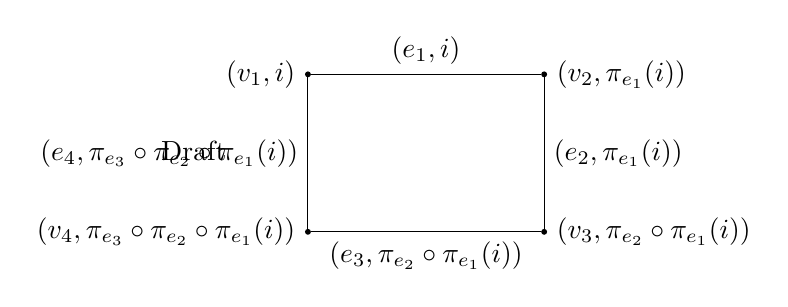
\begin{tikzpicture}
    % Nodes
    \node[draw, circle, fill=black, inner sep=0.6pt, label=left:{$(v_1,i)$}] (v1) at (0,2) {};
    \node[draw, circle, fill=black, inner sep=0.6pt, label=right:{$(v_2,\pi_{e_1}(i))$}] (v2) at (3,2) {};
    \node[draw, circle, fill=black, inner sep=0.6pt, label=right:{$(v_3,\pi_{e_2}\circ \pi_{e_1}(i))$}] (v3) at (3,0) {};
    \node[draw, circle, fill=black, inner sep=0.6pt, label=left:{$(v_4,\pi_{e_3}\circ\pi_{e_2}\circ \pi_{e_1}(i))$}] (v4) at (0,0) {};
    
    % Edges
    \draw (v1) -- node[above] {$(e_1,i)$} (v2);
    \draw (v3) -- node[right] {$(e_2,\pi_{e_1}(i))$} (v2);
    \draw (v3) -- node[below] {$(e_3,\pi_{e_2}\circ \pi_{e_1}(i))$} (v4);
    \draw (v4) -- node[left] {$(e_4,\pi_{e_3}\circ\pi_{e_2}\circ \pi_{e_1}(i))$} (v1);
\end{tikzpicture}
\end{center}
We can then define an index-$r$ covering map $p:\tilde{\mathcal S}\to \mathcal S$ acting on an element $(c,i)$ (vertex, edge or face) by $p((c,i))=c$, and therefore $p$ maps faces to faces. The inverse image of any vertex, edge or face is a set of $r$ vertices, edges or faces.\par

We now consider a square-complex $\mathcal S$, possibly with an empty set of faces, i.e. a graph. Given a covering $p:\tilde{\mathcal S}\to \mathcal S$, a \textit{deck transformation}\footnote{This name suggests an analogy to the mixing of a deck of cards, which are called sheets in the context of covering spaces.} is an automorphism $\psi:\tilde{\mathcal S}\rightarrow \tilde{\mathcal S}$ such that $p\circ \psi=p$. The set of deck transformations, endowed with the operation of composition of maps, forms a group denoted $\operatorname{deck}(p)$. It is called the \textit{group of deck transformations} and acts on the left on $\tilde{\mathcal S}$. A \textit{Galois covering} is a covering enjoying a left, free and transitive action of $\operatorname{deck}(p)$ on the fiber. For any Galois covering, $p:\tilde{\mathcal S}\rightarrow \mathcal S$, it can be shown that $\operatorname{deck}(p)\setminus \tilde{\mathcal S}\cong \mathcal S$.\par 
In the rest of this section, by a covering $p:\tilde{\mathcal S}\to \mathcal S$ we always mean a \textit{finite} \textit{connected} covering, i.e. one whose index is finite and for which $\tilde{\mathcal S}$ is also a connected complex. The following crucial results of this section apply in this context. \par

The theory of connected covering maps over a complex depends on the structure of its fundamental group in the following way. For every index $r$ subgroup $H $ of the fundamental group $\pi_1(\mathcal S)$ there exists an index $r$ covering $p:\mathcal S_H\to \mathcal S$, mapping the basepoint $\tilde v$ of $\mathcal S_H$ to $v$, and inducing an injective homomorphism $p_\#:\pi_1(\mathcal S_H,\tilde v)\to \pi_1(\mathcal S,v)$, such that $p_\#\pi_1(\mathcal S_H , \tilde v) = H$. A covering $p:\mathcal S_H\to \mathcal S$ is called \textit{Galois} or \textit{normal} when $H$ is a normal subgroup of $\pi_1(\mathcal S,v)$. All the coverings that we will study in Section \ref{section:New constructions of quantum Tanner codes} are of this form. It can be shown that, for such a covering map, we have the isomorphism $\operatorname{deck}(p)\cong\pi_1(\mathcal S,v)/H$. The most important result on coverings is the classification theorem known as the Galois correspondence, which we state in our restricted setting of finite index coverings of complexes with finitely many cells.\footnote{This theorem applies in a much broader context, but this is sufficient for our applications.}

\begin{theorem}[Galois correspondence]\label{Theorem Galois correspond}
For all $r\in \mathbb N$, there is a bijection between the set of basepoint-preserving isomorphism classes of index-$r$ connected covering spaces of a complex $\mathcal S$ and the set of index-$r$ subgroups of $\pi_1 (\mathcal S)$. Given such a covering $p:\tilde{\mathcal S}\to \mathcal S$, it is obtained by associating the subgroup $H=p_\#\pi_1 (\tilde{\mathcal S} )$ to the covering space $\tilde{\mathcal S}$. The index of the associated covering is equal to the index $[\pi_1(\mathcal S):H]$.
\end{theorem}
This theorem motivates our exhaustive searches of all possible Galois coverings in Section \ref{section:New constructions of quantum Tanner codes}. Using this correspondence, we also describe a procedure in Appendix \ref{appendix lift} specifically designed to generate the covering of a square complex associated to a given subgroup of its fundamental group.

\subsection{Tanner codes and their lifts}\label{section Tanner codes and their lifts}

In this section, we recall some definitions and set up notations related to linear codes. The central components of our quantum codes are classical Tanner codes. We review their construction and a method to lift them into larger codes.\par

We denote the parameters of a binary linear code $C\subseteq \mathbb{F}_2^n  $  as $[n,k,d]$, where $n$ its the length, $k$ its dimension and $d$ its distance, defined as $d=\min\limits_{c\in C\setminus \{0\} }|c|$. If $k=0$, our convention is to set $d=0$. In what follows, a linear code will be defined by the image of a linear map $g:\mathbb F_2^k\to \mathbb F_2^n$,  or the kernel of a linear map, $h:\mathbb F_2^n\to \mathbb F_2^m$, respectively represented in a preferred basis $B$ by a generator matrix $G:=\operatorname{Mat}_B (g)$, and a parity-check matrix $H:=\operatorname{Mat}_B (h)$. Given $x\in \mathbb F_2^n$, the vector $s=Hx$ is called the $syndrome$ of $x$.  The generator matrix of $C$ is the parity-check matrix of its dual $C^\perp=\{x\in \mathbb F_2^n\: :\: \forall c\in C, \langle x,c\rangle=0\}$. A code is called self-dual when $C^\perp=C.$\par

The central linear code construction of this article is the classical Tanner code of \cite{Tanner1981ARA}, which was made popular by Sipser and Spielman \cite{Sipser1996}.\par

Let $\mathcal G=(V,E)$ be a graph on $|E|=n$ edges. In the following $\mathbb{F}_2E:=\bigoplus_{e\in E}\mathbb{F}_2 e$ denote the space of formal linear combination of elements of the set $E$, playing the role of basis vectors. Given a vertex, $v$, the space $\mathbb F_2E(v)$, is the restriction of $\mathbb F_2E $ to the edge neighborhood of $v$. We define a set of binary \textit{local codes} $C_V:=(C_v )_{ v\in V}$ on the vertices of $\mathcal G$, where an element indexed by $v\in V$ is a code defined on the edge neighborhood of $v$, i.e. $C_v \subseteq \mathbb F_2E(v)$. For a vector $c\in \mathbb F_2 E$, we denote $c|_{E(v)} $ its restriction to the edge-neighborhood of $v$.
\begin{definition}[Classical Tanner code]\label{definition classical Tanner code}
Let $\mathcal G=(V,E)$ be a graph and $C_V=(C_v )_{ v\in V}$ be a set of binary local codes. We define the Tanner code associated to $\mathcal{G}$ and $C_V$ as
\[ T(\mathcal G,C_V)=\{ c\in \mathbb F_2E : c|_{E(v)}\in C_v\text{ for all }v\in V\}.\]
\end{definition}

A Tanner code can also be defined by the kernel of a parity-check matrix. Suppose that $C_v$ is the kernel of a map $h_v:\mathbb F_2E(v)\to \mathbb F_2^{m_v}$ and let $i_v: \mathbb F_2^{m_v}\to \bigoplus_{u\in V} \mathbb F_2^{m_u}$ be the canonical linear embedding map. The Tanner code $C=T(\mathcal G,C_V)$ is the kernel of the map $
h :\mathbb F_2 E\xrightarrow[]{} \bigoplus_{u\in V} \mathbb F_2^{m_u}$, defined on an edge between vertex $v$ and $w$ by
\begin{equation}\label{equation:tanner code map}
h (e)= i_v\circ h_v (e) + i_w\circ h_w (e),
\end{equation}
and extended by linearity over $\mathbb F_2 E$. All vector spaces being given with a prefered basis, $h_v$ can be represented by a matrix $H_v$ and $h$ by a matrix $H$. Denoting $w$, $w_v$, the maximum row-weight of $H$ and $H_v$, respectively, and $q,q_v$ their column-weight, we have \[ w=\max\limits_{v\in V }w_v, \quad \quad q\leq\max \limits_{ \{v,w\}\in E} q_v+q_w .\]
For linear codes, lifting is an operation of major interest that produces families of LDPC codes \cite{Thorpe2003}, possibly with linear dimension and distance. It is equivalent to a covering of the Tanner graph representation of the code. In this article, we focus on lifts of Tanner codes. In that case, out of the many possible lifts, there exists a preferred choice, that we call the \textit{lift of a Tanner code}, as we will not use other types of lifts. From now on, we consider a graph $\mathcal G$ that has no loops. Then, given a graph covering $p:\tilde{\mathcal G}\to \mathcal  G$, where $\tilde{\mathcal G}=(\tilde V,\tilde E)$, the linear extension $p_*$ of $p$ on the set of edges induces an isomorphism\footnote{In the context of coverings of cells complexes, $p_*$ acts on chains of  $\mathbb F_2\tilde E$ and $\mathbb F_2\tilde V$  in the cellular chain complex and is a chain map.} $\mathbb F_2\tilde E(\tilde v)\overset{p_*}{\cong} \mathbb F_2 E(v)$, for any $\tilde v\in p^{-1}(v)$, which by definition sends basis vectors to basis vectors, i.e. edges to edges. 
\begin{definition}[Lift of Tanner code]\label{definition Lift of classical Tanner code}
 Let $C=T(\mathcal G,C_V)$ and $p:\tilde{\mathcal G}\to \mathcal  G$ be a graph covering, with $\tilde{\mathcal G}=(\tilde V, \tilde E)$. For each vertex $\tilde {v}\in \tilde V$, we associate the code $C_{\tilde v}\subseteq \mathbb F_2E(\tilde v)$, such that $C_{\tilde v} \overset{p_*}{\cong} C_{p(v)}$. The lifted Tanner code associated to $p$ is the code $\tilde C=T(\tilde{\mathcal G},C_{\tilde V})$, where $C_{  \tilde V}= (C_{\tilde v})_{ \tilde v\in \tilde V}$. In other words,
\[ T(\tilde{\mathcal G},C_{\tilde V})=\{c\in \mathbb F_2 \tilde E \: :\: p_*(c|_{\tilde E(\tilde v)})\in C_{p(\tilde v)}, \text{for all }\tilde v\in \tilde V\} \]
\end{definition}
Using the notations of the previous definitions, suppose that for each $v\in V$, $C_v$ is the kernel of a map $h_v$ represented by a matrix $H_v$, as described below Equation \eqref{equation:tanner code map}. Given a complete parity-check matrix $H$ of the Tanner code $C$, we can construct a Tanner graph of $C$. In this context, by lifting we always mean that for any $\tilde v\in p^{-1}(v)$, we define the code $C_{\tilde v}$ as the kernel of a map $h_{\tilde v}$ represented by the matrix $H_{\tilde v}=H_v$. In this way, fixing a matrix representation $H$ induces a matrix representation $\tilde H$, the parity-check matrix of $\tilde C$, up to permutation of the rows. Denoting $\tilde w$, $\tilde q$ the maximum row and column-weight of $\tilde H$, we have that \begin{equation}\label{Equation: lift conserve degree}
    \tilde q=q, \quad \tilde w=w.
\end{equation}
This can also be deduced from the fact that the lift of a Tanner code is an example of lift of a classical code associated to a certain covering, not necessarily connected, over the Tanner graph associated to $H$.\par

An automorphism of a binary linear code $C$ is a permutation of the coordinates mapping $C$ to itself. The set of automorphisms of $C$ forms the group $\operatorname{Aut}(C)$.  In the case of a lifted Tanner code $\tilde C$, notice that the group of deck transformation of $p:\tilde{\mathcal G}\to \mathcal  G$ is a symmetry group of the Tanner graph associated to the parity-check matrix $\tilde H$ described above. Therefore, given an element $\psi \in \operatorname{deck}(p)$, a vector $x\in \mathbb F_2 \tilde E$ with syndrome $\tilde Hx=s$, there exists a permutation $\sigma$ of the syndrome coordinates such that $\tilde H\psi(x)=\sigma(s)$. As so, $ \operatorname{deck}(p)$ is a subgroup of $\operatorname{Aut}(\tilde C)$, with the property that each element in this subgroup is equivalent to a certain permutation of the checks.

\subsection{Local codes}\label{section:local codes}

Throughout this article, for an integer $\ell\geq 1$, we denote $[\ell]= \{ 0,\dots ,\ell-1\}$. The classical local codes that will constitute our Tanner codes are built as dual of tensor-product codes. The tensor-product of linear codes $C\subseteq \mathbb F_2^{\ell_C}$ and $D\subseteq \mathbb F_2^{\ell_D}$, is the linear code denoted $ \Pi=C\otimes D\subseteq \mathbb F_2^{\ell_C}\otimes \mathbb F_2^{ \ell_D}$. The canonical bases of $ \mathbb F_2^{\ell_C}$ and $\mathbb F_2^{\ell_D}$ are indexed by the elements of $[\ell_C]$ and $[\ell_D]$, respectively. These bases naturally induce the canonical product basis for $\mathbb F_2^{\ell_C}\otimes \mathbb F_2^{ \ell_D}$, whose elements are indexed by $[\ell_C]\times[\ell_D]$. In this basis, the codewords of the product code can be seen as the matrices all of whose rows and columns are, respectively, codewords of $C$ and $D$. The dual of the tensor-product is \[ \Pi^\perp=C^\perp\otimes \mathbb F_2^{\ell_D}+  \mathbb F_2^{\ell_C}\otimes D^\perp.\]
In the tensor codes considered later, one of the factor is a repetition code of length $2$ and the other one is either a cyclic or a double-circulant code. We therefore recall some essential facts about these two types of codes, taken from \cite{MacWilliamsSloane}.\par

A binary cyclic code ${C} \subseteq \mathbb F_2^\ell$ is a code that is stable under the action of the automorphism $\rho :\mathbb  F_2^\ell \to  \mathbb F_2^\ell, (c_0, \ldots, c_{\ell-1})\mapsto(c_{\ell-1},c_0 \ldots, c_{\ell-2}) $.\par
A practical way to define a cyclic code is to identify $\mathbb F_2^\ell$ and the polynomial ring $ R_\ell:=\mathbb F_2[X]/{(X^\ell-1)}$, using the $\mathbb F_2$-linear isomorphism \[ \varphi: R_\ell \longrightarrow \mathbb F_2^\ell,\quad  g_0 + g_1 X + \cdots + g_{\ell-1}X^{\ell-1}  \longmapsto 
  (g_0, \ldots,g_{\ell-1}).\]
In $ R_\ell$, the transformation corresponding to the rotation $\rho$ is multiplication by $X$. A code $C\subseteq R_\ell$ is cyclic if it is stable under this operation, and by linearity it is an ideal of $R_\ell$. These ideals are in one-to-one correspondence with the divisors of $X^\ell-1$. Given $g \in \mathbb F_2 [X]$ such that $g ~|~ X^\ell-1$, the code $\mathscr{C}_\ell (g)$ is defined as the code equal to the ideal generated by $g$, and $g$ is referred the \textit{generating polynomial} of the code. It is well-known that $\mathscr{C}_\ell (g)$ has dimension $\ell-\deg (g)$.\par

The dual of a cyclic code is cyclic and its generating polynomial can be obtained as follows. Given a polynomial $h\in R_\ell$, let $\bar{h} := X^{\deg h}h(1/X)$ denote the reciprocal polynomial of $h$. Over $\mathbb F_2$, $X^\ell - 1$ is equal to its reciprocal polynomial so, if $h~|~X^\ell-1$, then $\bar{h}~|~X^\ell-1$. Letting $h$ be the polynomial such that $gh = X^\ell-1$, also called the check-polynomial, we have  $\mathscr{C}_\ell (g)^{\bot} = \mathscr{C}_\ell (\bar h)$.\par

Given any polynomial $f\in R_\ell$, we define $\mathbb G(f)$ as the circulant matrix whose first row is $\varphi(f)$. Note that $G=\mathbb G(g)$ is a square generator matrix of the code. The row-weight of $G$ is hence directly given by the weight of $g$, i.e. its number of non-zero coefficients.\par

The second type of linear codes considered in the tensor-product are double-circulant codes. They are a subclass of quasi-cyclic codes, built from any polynomial $f\in R_\ell$. The double-circulant code $\mathscr{D}_{2\ell}(f)\subseteq \mathbb F_2^{2\ell}$ is defined as the image of the generator matrix \[G= \left[\begin{array}{c|c} 
 \mathbb G(1) & \mathbb G(f) \end{array}\right],\]
where $\mathbb G(1)$ corresponds to the $\ell\times\ell$ identity matrix. In Section \ref{section:Quantum Tanner code with double-circulant local code}, the ambient space $\mathbb F_2^{2\ell}$ of a double-circulant code $\mathscr{D}_{2\ell}(f)$ is always understood to be given with the canonical basis indexed by the columns of the generating matrix given in the above form. It is important to note that the code generated by $G$ is invariant under simultaneous cyclic permutation within the left and right blocks. That is, $\mathbb Z_\ell$ is a subgroup of the automorphism group $\operatorname{Aut}(\mathscr{D}_{2\ell}(f))$. The dual of $\mathscr{D}_{2\ell}(f)$ is generated by the matrix \[ H=\left[\begin{array}{c|c} 
 \mathbb G(\bar f)&\mathbb G(1)   \end{array}\right],\]
and is also invariant under simultaneous cyclic permutation within the left and right blocks.

\section{Quantum Tanner codes and their lifts}\label{section: quantum Tanner codes and their lifts}

\subsection{Quantum Tanner codes}\label{section Quantum Tanner codes}

CSS codes are instances of stabilizer quantum error correcting codes, which first appeared in the seminal work of Calderbank, Shor and Steane \cite{Calderbank1996,Steane1996,Stean1996Multiple}. Let $C_X$ and $C_Z$ be two linear codes with parity-check matrices $H_X$ and $H_Z$, such that $C_X^\perp\subseteq C_Z$, referred to as the \textit{orthogonality condition}. The CSS code $\text{CSS}(C_X,C_Z)$ is the subspace \[\operatorname{Span}\left \{\sum_{z\in C_Z^\perp }\ket{x+z}\text{ } \: :\:\text{ } x\in C_X \right \}\]
of $(\mathbb{C}^2)^{\otimes n}$. Its parameters, denoted $[[n,k,d]]$, are \textit{its length} $n$, \textit{dimension} $k = \dim(C_X / C_Z^\perp)$ and \textit{distance} $d$. The latter is defined as $d := \min(d_X, d_Z)$, with 
\[d_X=\min\limits_{c\in C_Z\setminus C_X^\perp}|c|, \quad 
d_Z=\min\limits_{c\in C_X\setminus C_Z^\perp}|c|.\] The maximum row weight and column weight in the parity check matrix $H_X$, respectively $H_Z$, are denoted $w_X,q_X$, respectively $w_Z, q_Z$. We denote $W:=\operatorname{max}(w_X,q_X,w_Z,q_Z)$. A family of codes is called \textit{Low Density Parity Check} (LDPC) if $W$ is upper bounded by a constant. If $k=0$, our convention is to set $d=0$.\par

The only CSS codes that we consider in this article are \textit{quantum Tanner codes}, a type of codes introduced by Leverrier and Z\'emor \cite{Leverrier2022}, in which $C_X,C_Z$ is a pair of classical Tanner codes.\par 

A practical way to build two Tanner codes $C_X$ and $C_Z$ satisfying the orthogonality condition is to generate them simultaneously by considering two specific graphs embedded in a square-complex. Let $\mathcal S:=(V,E,F)$ be a bipartite square-complex and denote the partition $V=V_X \sqcup V_Z$. As remarked in \cite{Leverrier2022}, if we restrict the vertex set to $V_X$, each square face is now incident to only two vertices, in its opposite corners. The set of squares $F$ can now be seen as a set of edges on $V_X$, and therefore it defines a graph that we denote by $\mathcal G_X^\Box=(V_X,F)$ and call the \textit{diagonal graph} on $V_X$. Similarly, restricting the vertex set to those of $V_Z$, we obtain the diagonal graph $\mathcal G_Z^\Box=(V_Z,F)$. These graphs can then be treated as the graph components of two classical Tanner codes whose set of bits are identified with $F$, and as so we can identify the ambient space of these codes as $\mathbb F_2F$. However, to fully define these codes, it remains to coherently assign local codes $C_{V_X},C_{V_Z}$ to the vertices of the graphs $\mathcal G_X^\Box$, $\mathcal G_Z^\Box$, in order to obtain the Tanner codes 
\[ C_X=T(\mathcal G_X^\Box, C_{V_X} ), \quad C_Z=T(\mathcal G_Z^\Box, C_{V_Z}),\]
such that $C_X^\perp\subseteq C_Z$. This procedure is better carried out case by case, and will be  undertaken in Section \ref{section:New constructions of quantum Tanner codes} on explicit square-complexes.\par

\subsection{Lifting quantum Tanner codes}\label{section lift of quantum Tanner codes}
We now describe a lifting procedure for quantum Tanner codes, which generalizes the lift of \cite{guemard2024liftsquantumcsscodes}. The approach is an extension of the method applied in \cite{Panteleev2021} to design a family of Sipser-Spielman codes \cite{Sipser1996}, with optimal parameters. Here, we use a covering of a bipartite square-complex in order to create one for each of its two diagonal graphs.\par

Suppose that $\operatorname{CSS}(C_X, C_Z)$ is a quantum Tanner code, built over a bipartite square-complex $\mathcal S=(V=V_X\sqcup V_Z,E,F)$, with $C_X=T(\mathcal G_X^\Box, C_{V_X} )$ and $C_Z=T(\mathcal G_Z^\Box, C_{V_Z})$. Given a covering map $p:\tilde{\mathcal S} \to \mathcal S$, the 1-skeleton of $\tilde{\mathcal S}=(\tilde V,\tilde E,\tilde F)$ is also bipartite with bipartition $\tilde V=\tilde V_X\sqcup \tilde V_Z$, where $\tilde V_X=p^{-1}(V_X)$ and $\tilde V_Z=p^{-1}(V_Z)$. We can hence consider the diagonal graphs $\tilde{\mathcal G}_X^\Box=(\tilde V_X,\tilde F)$ and $\tilde{\mathcal G}_Z^\Box=(\tilde V_Z,\tilde F)$. \par

Using the notation above, we have the following lemma.
\begin{lemma}\label{lemma restriction covering map}
The covering map $p$ induces two covering maps $p_X: \tilde{\mathcal G}_X^\Box \to \mathcal G_X^\Box $ and $p_Z:\tilde{\mathcal G}_Z^\Box \to \mathcal G_Z^\Box$. If $p$ is a Galois covering map, then $p_X$ and $p_Z $ are also Galois.
\end{lemma}
\begin{proof}
Suppose that $p:\tilde{\mathcal S}\rightarrow  \mathcal S$ 
 is an index-$r$ covering defined by an assignment of permutations to all the oriented edges of $\mathcal S$, i.e $\pi_e\in S_r$ for $r>0$ such that $\pi_{e^{-1}}=\pi_{e}^{-1}$. It is essential to note that $\tilde V_X=p^{-1}(V_X)$, $\tilde V_Z=p^{-1}(V_Z)$, and $\tilde F =p^{-1}(F)$, so that we have $r$ vertices or faces in $ \tilde{\mathcal G}_X^\Box$ projected by $p$ onto each vertex or face in $ \mathcal G_X^\Box$, and similarly for the diagonal graph on $V_Z$. We now need to show that these cells are assembled into coverings of the diagonal graphs.\par
 Given a face $f\in F$ described by the path $e_1.e_2.e_3.e_4=[v_1,v_2].[v_2,v_3].[v_3,v_4].[v_4,v_1]$, then for all $i\in [r]$, the face labeled $(f,i)$ in $\tilde{\mathcal S}$ can be defined by the 4-cycle as described in Section \ref{section covering maps}. Therefore, if $e=[v_1,v_3]$ is an edge in $\mathcal G_X^\Box$, then an edge $(e,i)$ in the covering $\tilde{\mathcal G}_X^\Box$, projected onto $e$ by $p$, is written $[(v_1,i), (v_3,\pi_{e_2}\circ \pi_{e_1}(i))]$. Let us assign the permutation $\pi_{e_2}\circ \pi_{e_1}\in S_r$ to $e$. We can similarly assign a composition of two permutations to each diagonal edge of $\mathcal G_X^\Box$, according to the corresponding square in $\mathcal S$. This defines a covering map $p_X: \tilde{\mathcal G}_X^\Box \to \mathcal G_X^\Box $. A similar procedure on $\tilde{\mathcal G}_Z^\Box$ defines a covering map $p_Z:\tilde{\mathcal G}_Z^\Box \to \mathcal G_Z^\Box$.\par
If $p:\tilde{\mathcal S}\to \mathcal S$ is a Galois covering, then $\tilde{\mathcal G}_X^\Box$ inherits the free transitive action of the group $\operatorname{deck}(p)$, since we can see $p_X$ as a restriction of $p$ on the vertices and on the diagonal of the faces in $\tilde{\mathcal G}_X$. Therefore, $p_X: \tilde{\mathcal G}_X^\Box\to \mathcal G_X^\Box$ is also a Galois covering with a group of deck transformations $\operatorname{deck}(p)$, and similarly for $p_Z$.
\end{proof}

\begin{remark}
If $p$ is a connected covering, then $p_X$ and $p_Z$ are also connected coverings. Indeed, if two faces are adjacent in $\tilde{\mathcal S}$, then their induced edges in any of the two diagonal graphs must also be adjacent, and using this argument for any two distant faces in $\tilde{\mathcal S}$ shows that any two edges in the diagonal graphs are connected by a path.
\end{remark}

We now have all the elements to define the lift of a quantum Tanner code, using the lift of classical Tanner codes of Definition \ref{definition Lift of classical Tanner code}.

\begin{definition}[Lift of quantum Tanner code]\label{definition Lift of quantum Tanner code}
Let $\tilde C_X=T(\tilde{\mathcal G}_X^\Box ,C_{\tilde V_X})$ and $\tilde C_Z=T(\tilde{\mathcal G}_Z^\Box ,C_{\tilde V_Z})$ be lifted Tanner codes associated to $p_X$ and $p_Z$, as above, of $C_X=T(\mathcal G_X^\Box, C_{V_X} )$ and $C_Z=T(\mathcal G_Z^\Box, C_{V_Z})$, and satisfying $\tilde C_X^\perp\subseteq \tilde C_Z$. We define the lifted quantum Tanner code associated to $p$ as the code $\operatorname{CSS}(\tilde C_X,\tilde C_Z)$.
\end{definition}

This definition suggests that the lifted classical Tanner codes associated to $p_X$ and $p_Z$ do not always satisfy the orthogonality condition. This depends on certain properties of the complex $\mathcal S$, and on the choice of local codes. However, there are cases where they always do, as shown below.

\begin{proposition}
    Let $\operatorname{CSS}(C_X,C_Z)$ denote a quantum Tanner code over a bipartite square-complex $\mathcal{S}$, for which the star of every vertex has a simply connected closure. Then the lifting procedure above, applied to every finite covering space, $p:\tilde{\mathcal{S}}\to \mathcal{S}$, defines a valid CSS code.
\end{proposition}
\begin{proof}
    The star of every vertex having a simply connected closure, the support intersection between a check of $\tilde C_X$ and one of $\tilde C_Z$, associated to two incident vertices of $\tilde{\mathcal S}$, is isomorphic to the support intersection of their projection in $\mathcal S$ by the covering map.
\end{proof}
Hereafter, we define quantum Tanner code families beyond this restriction on $\mathcal S$.\par

In this work, an automorphism of a quantum code $\mathcal Q=\operatorname{CSS}(C_X,C_Z)$ is defined as a permutation of the coordinates of the qubits which is equivalent to a permutation of the parity checks of both $H_X$ and $H_Z$. The set of automorphisms of $\mathcal Q$ forms the group $\operatorname{Aut}(\mathcal Q)$. The automorphism group of a quantum code is known to be related to the set of logical Clifford operations implementable on the code in a fault-tolerant way \cite{Breuckmann2024foldtransversal}.\par

In the case of a lifted quantum Tanner code $\tilde{\mathcal Q} $, notice that the group of deck transformation of $p:\tilde{\mathcal S}\to \mathcal  S$ is a symmetry group of the Tanner graph of the quantum code. It is also a symmetry group of each of the Tanner graphs associated to $\tilde H_X$ and $\tilde H_Z$. Thus, given an element\footnote{The action of $\psi$ is naturally extended to the $\mathbb F_2$-space of the lifted codes} $\psi \in \operatorname{deck}(p)$, a vector $c\in \mathbb F_2 \tilde F$ with syndrome $\tilde H_Xc=s_X$ and $\tilde H_Zc=s_Z$ , there exist two permutations $\sigma_X$ and $\sigma_Z$ of the syndrome coordinates such that $\tilde H_X\psi(c)=\sigma_X(s_X)$ and $\tilde H_Z\psi(c)=\sigma_Z(s_Z)$. Therefore, $ \operatorname{deck}(p)$ is a subgroup of $\operatorname{Aut}(\tilde{\mathcal Q})$.

\section{New constructions of quantum Tanner codes}\label{section:New constructions of quantum Tanner codes}

\subsection{General procedure}\label{section:general procedure}

In this section and the next, we introduce new codes constructed by lifting short quantum Tanner codes. As described previously, to define a short code, we need a square-complex and a set of local codes associated to its vertices. The possibility of lifting a code is governed by Theorem \ref{Theorem Galois correspond}, and for the purpose of generating families of lifted codes, the square complex must have a fundamental group with infinitely many finite-index subgroups. Our strategy is to select a group $G$ and construct a bipartite square-complex $\mathcal S$ which has $G$ for fundamental group, and has a local product structure. In Section \ref{section:Quantum Tanner code with cyclic local code} and Section \ref{section:Quantum Tanner code with double-circulant local code}, we obtain $\mathcal S$ by cellulating the presentation complex of a finitely-presented group, or a homotopy equivalent space. \par

We first describe the construction of a presentation complex, as exposed in \cite{HatcherTopo}. Let $G=\langle S |  R\rangle$ be a group presentation, where $S$ is the set of generators denoted $g_i$ and $R$ the set of relations denoted $r_j$. $G$ is the quotient of a free group $F_{|S|}$ on the generators of $S$ by the normal closure of the group generated by $R$. The relations of $R$ are the generators of the kernel of the map $F_{|S|}\to G$. For any group presentation, we can utilize this quotient structure to construct a two-dimensional cell complex $M_G$, called the \textit{presentation complex} of $G$, having 1 0-cell, $|S|$ 1-cells and $|R|$ 2-cells, and such that $\pi_1(M_G)=G$. To construct it, we start from its 1-skeleton: the wedge of circles $\vee_i S_i^1$ attached to a vertex $v$ and consists of edges $e_{g_i}$ that are directed loops. This gives a space with fundamental group $F_{|S|}$. A relation is a product of the generators and it specifies a circuit in the graph. For each relation $r_j$, we attach one 2-cell, labeled $f_j$, along the circuit specified by $r_j$. For example, if $r_j=g_i g_j\dots g_k$, then we attach a face along the circuit $e_{g_i}\cdot e_{g_j}\dots e_{g_k}$. The effect is to trivialize the element of $F_{|S|}$ corresponding to $r_j$. \par 

We will focus on group presentations with 2 generators and 1 relation. As such, all of their associated presentation complexes have 2 edges and 1 face.  It is, however, important to note that these 2D spaces are not square-complexes in general. Given one of these groups, $G$, by subdividing the face of its presentation complexes, or a homotopy equivalent space, into squares, we will be able to obtain a bipartite square-complexes $\mathcal S=(V=V_X\sqcup V_Z,E,F)$ that has locally the structure of a product space.\par

From the diagonal graphs of $\mathcal S$, and a choice of local linear codes, it is possible to generate Tanner codes $C_X=T(\mathcal G_X^\Box, C_{V_X} )$ and $C_Z=T(\mathcal G_Z^\Box, C_{V_Z})$, satisfying $C_X^\perp\subseteq C_Z$. They will be chosen to have a symmetry group adapted to the local product structure of $\mathcal S$ and to its periodic boundary conditions. These will be dual of tensor-product of cyclic or double-circulant codes. \par

Lastly, new square-complexes will be obtained by considering connected Galois covering spaces, such as $p:\tilde{\mathcal S}\to \mathcal S$. By restricting $p$ to $\mathcal G_X^\Box$ and $\mathcal G_Z^\Box$, we define the covering maps  $p_X: \tilde{\mathcal G}_X^\Box \to \mathcal G_X^\Box $ and $p_Z:\tilde{\mathcal G}_Z^\Box \to \mathcal G_Z^\Box$, which are also connected and Galois, as discussed in Section \ref{section lift of quantum Tanner codes}. We then use the procedure of Definition \ref{definition Lift of quantum Tanner code} to lift $\operatorname{CSS}(C_X,C_Z)$. Recall that for each lift, the group of deck transformation is a subgroup of the automorphism group of the corresponding code.\par

To compute subgroups and quotient groups of $G$, needed for the Galois covering-space constructions, we use the GAP package LINS \cite{GAP4}.  As we are interested in short codes, we only compute normal subgroups up to index 30. To compute an upper bound on the distances $d_X $ and $d_Z$ of $\operatorname{CSS}(\tilde C_X,\tilde C_Z)$, we use the GAP package QDistRnd \cite{Pryadko2022}.

\subsection{ Quantum Tanner code with cyclic local code}\label{section:Quantum Tanner code with cyclic local code}

\begin{figure*}[t]
  \centering
  \includegraphics[scale=1]{Quantum_Tanner_L.pdf}
  \caption{Left: space homotopy equivalent to the presentation complex of $\operatorname{L}(3)$. Right: its subdivision into a square-complex and the indexing of the faces by $(i,j)\in [2]\times [\ell]$.}
  \label{fig:Quantum_Tanner_L}
\end{figure*}

Our first example of quantum Tanner code is obtained by considering a space homotopy equivalent to the presentation complex of the group \[\operatorname{L}(\ell)=\langle a,b | a^\ell b^{-\ell}\rangle,\]
combined with a set of local tensor-product codes of length $2\ell$, and their dual. \par
This space is shown in Figure \ref{fig:Quantum_Tanner_L} for $\ell=3$. We build a square-complex by subdividing each horizontal edge into 2 edges. We also connect the new vertices by additional vertical edges, which may be multi-edges, hence subdividing the unique face. This forms the bipartite square-complex $\mathcal S_\ell=(V=V_X\sqcup V_Z,E,F)$ which has $|V|=4$, $|E|=2\ell+4$, and $|F|=2\ell$. The subdivision for $\ell=3$ is also shown in Figure \ref{fig:Quantum_Tanner_L}. Notice that the 1-skeleton of this complex is a bipartite multi-graph, which is sufficient to use it for a quantum Tanner code construction.\par

We index the faces of this complex by the product set $[2]\times [\ell]$, where the index $(i,j)$ corresponds to the face in the $(i+1)\cdot (j+1)$-th position, when counting from left to right in Figure \ref{fig:Quantum_Tanner_L}. We can see that each vertex is incident to all the $2\ell$ faces. The associated $2\ell$ edges of the diagonal graphs $\mathcal G_X^\Box $ and $\mathcal G_Z^\Box$ inherits the indexing of the faces of $\mathcal S_\ell$.\par

To construct the local code, we first consider $\mathscr{C}_2(1+X)$, the repetition code of length $2$, and $\mathscr{C}_\ell(g)$, the cyclic code of length $\ell$ generated by $g$. We define the tensor code $ \Pi_X, \Pi_Z\subseteq \mathbb F_2^{2}\otimes\mathbb F_2^{\ell}$, where 
\begin{align*}
    \Pi_X&=\mathscr{C}_2(1+X)\otimes\mathscr{C}_\ell(g), \\
    \Pi_Z&=\mathscr{C}_2(1+X)\otimes\mathscr{C}_\ell(g)^\perp,
\end{align*}
and $\mathbb F_2^{2}\otimes\mathbb F_2^{\ell}$ is endowed with the canonical product basis indexed by $[2]\times [\ell]$, as described in Section \ref{section:local codes}.\par

We start by defining a classical Tanner code associated to $\mathcal G_X^\Box$. The graph $\mathcal G_X^\Box=(V_X,F)$ has only two vertices, $V_X=\{x_{0},x_{1}\}$, as shown in Figure \ref{fig:Quantum_Tanner_L}. The edge-neighborhood of these vertices, in the graph, is equal to their face-neighborhood in the complex $\mathcal S$, and $F(x_{0})=F(x_{1})=F$. Each local code associated to these vertices is set to be isomorphic to the dual of the tensor code $C_{x_t}\cong \Pi_X^\perp$, $t=0,1$. For $t=0$, the isomorphism is induced by the isomorphism $\phi_{x_0}:\mathbb F_2 F \to \mathbb F_2^{2}\otimes\mathbb F_2^{\ell}$ sending edges to the canonical basis vectors. For simplicity, we describe this map by its action on the indexing of the basis elements, i.e. the faces, which is given by
\begin{align*}
    (i,j)&\mapsto (i,i+j \operatorname{mod} \ell),
\end{align*}
where our choices of indexing for basis elements in the case of product codes and cyclic codes are described in Section \ref{section:local codes}. The bijection $\phi_{x_1}:\mathbb F_2 F \to \mathbb F_2^{2}\otimes\mathbb F_2^{\ell}$ is determined by the identity mapping on this indexing
\begin{align*}
    (i,j)&\mapsto (i,j).
\end{align*}
This completes the characterization of the local codes $C_{V_X}=(C_{x_i})_{i\in\{0,1\}}$ and of the classical Tanner code $C_X:=T(\mathcal G_X^\Box,C_{V_X})$.\par

The classical Tanner code associated to $\mathcal G_Z^\Box$ is defined similarly. The graph $\mathcal G_Z^\Box=(V_Z,F)$ also has two vertices, $V_Z=\{z_{0},z_{1}\}$, which are incident to all the faces, i.e.  $F(z_{0})=F(z_{1})=F$. Each local code associated to these vertices is set to be isomorphic to the dual of the same tensor code, $C_{z_t}\overset{\phi_{z_t}}{\cong }\Pi_Z^\perp$ where each isomorphism is induced by $\phi_{z_t}=\phi_{x_t}$, for $t=0,1$. This completes the characterization of $C_{V_Z}=(C_{z_i})_{ i\in \{0,1\}}$ and $C_Z:=T(\mathcal G_Z^\Box,C_{V_Z})$.\par

We now explain in words why the code $\mathcal Q=\operatorname{CSS}(C_X,C_Z)$ is well-defined. The first factor of each product code $\Pi_X,\Pi_Z$ is a repetition code to ensure that the checks associated with $x_0 $ and $x_1$ commute with the checks associated to the vertices $z_1$ and $x_0$, respectively. Moreover, due to the identification of the left and right edges of the presentation complex, the linear codes need to have a cyclic symmetry,  in order for a check associated to $x_0$ to commute with one associated to $z_1$. This is why the second factor in $\Pi_X$ and $\Pi_Z$ can be, respectively, a cyclic code and its dual to ensure $C_X^\perp\subseteq C_Z$.  In fact, this constraint is too strong for commutativity here, but it becomes necessary when the code is lifted.\par

Another way to describe $C_X$ and $C_Z$ is by the kernel of a parity-check matrix $H_X$ and $H_Z$, as explained in Section \ref{section Tanner codes and their lifts}. We denote $h$ the check polynomial of $\mathscr{C}_\ell(g)$. In a certain basis, the parity check matrix can be written
\begin{align*}
     H_X=\left[\begin{array}{c|c} 
 \mathbb G( Xg(X))  &  \mathbb G (g(X))\\ \hline
 \mathbb G (g(X)) &  \mathbb G( g(X))
\end{array}\right], \quad \quad
H_Z=\left[\begin{array}{c|c} 
 \mathbb G( \bar h(X))  &  \mathbb G (\bar h(X))\\ \hline
 \mathbb G (X\bar h(X)) &  \mathbb G( \bar h (X))
\end{array}\right].
\end{align*}
   
It is direct to verify that $H_X\cdot H_Z^T=0$, using that $\mathbb G( Xg(X))$ is a cyclic permutation of $\mathbb G( g(X))$.\par

Now that we have described quantum Tanner codes constructed on the square-complex $\mathcal S_\ell$, we can consider their lifts, as in Definition \ref{definition Lift of quantum Tanner code}. Our first objective is to prove that our construction behaves well under lifting.
\begin{proposition}
    Let $p:\tilde{\mathcal S}_\ell\to \mathcal S_\ell$ be a covering map and $\tilde C_X=T(\tilde{\mathcal G}_X^\Box ,C_{\tilde V_X})$, $\tilde C_Z=T(\tilde{\mathcal G}_Z^\Box ,C_{\tilde V_Z})$, the lifted classical Tanner codes associated to $p$. Then $\tilde C_X^\perp\subseteq \tilde C_Z$.
\end{proposition}
\begin{proof}
The idea is to determine the intersection of the face neighborhood $F(\tilde x_s)\cap F(\tilde z_t)$, for any pair of vertices $\tilde x_s\in p^{-1}(x_s)$ and $\tilde z_t\in p^{-1}(z_t)$, $s,t\in \{0,1\}$, and show that the support intersection of any $X$ and $Z$ checks associated to these vertices is of even size. By symmetry of the code, it is sufficient to verify this condition for pairs $(\tilde x_0,\tilde z_0)$ and $(\tilde x_0,\tilde z_1)$ in $\tilde S_\ell$.\par
It is clear that any adjacent vertices $\tilde x_0,\tilde z_0$ share at least 2 faces, which are attached to an edge $\tilde e=\{\tilde x_0,\tilde z_0\}$, drawn vertically on Figure \ref{fig:Quantum_Tanner_L}. Since a $X$-check is a codeword of the product code $\Pi_X$, if it acts on the qubit associated to one of the two faces, then it must also act on the other, and similarly for a $Z$-check. Therefore, the support of an $X$ and $Z$ check associated to the vertices $\tilde x_0 $ and $\tilde z_0$, respectively, must intersect on an even number of qubits.\par
A pair of adjacent vertices of the form $\tilde x_0,\tilde z_1$ are connected by an edge incident to $\ell$ faces in $\tilde S_\ell$. The support vector of an $X$-check associated $\tilde x_0$ is a codeword of $\mathscr{C}_\ell(g)$, while the support vector of a $Z$-check associated $\tilde z_1$ is a codeword of $\mathscr{C}_\ell(g)^\perp$. These vectors being orthogonal, their support intersection is even.
\end{proof}

\begin{table}[]
\centering 
\begin{tabular}{l|l|l|l|l|l}

$\ell$&  $W$&lift index& $\operatorname{deck}(p)$& $[[n,k,d]]$   &$d^2/n$\\
\hline \hline 
 10& 4& 1& $1$&$[[20,2,2]]$ &0.2\\
 & & 20& $D_{20}$, $\mathbb Z_5 \rtimes \mathbb Z_4$&$[[400,2,20]]$ &1\\ \hline   
  14&     12 &1     &   $1$&                     $[[28,2,6]]$ &1.25\\
 & & 4& $\mathbb Z_2 \times \mathbb Z_2$, $\mathbb Z_4$&$[[112,2,12]]$ &1.25\\
 & & 7& $\mathbb Z_7$&$[[196,2,18]]$ &1.65\\
 & & 16& $\mathbb Z_4 \rtimes \mathbb Z_4$, $\mathbb Z_8 \rtimes \mathbb Z_2$, $Q_{16}$&$[[448,2,24]]$           &1.25\\ 
  &          &28&       $\mathbb Z_{28}$&                     $[[784,2,36]]$ &1.65\\

\end{tabular}
\caption{Parameters of selected lifted quantum Tanner codes built from the space of Figure \ref{fig:Quantum_Tanner_L}, with homotopy group $\operatorname{L}(\ell)$. Different groups in an entry of the 4th column correspond to different lifted codes with the same parameters. Here, $W$ denotes the maximum row or column-weight of the parity-check matrices. The value of $d$ is an upper bound found with the GAP package \cite{Pryadko2022}, and in all these cases $d_X=d_Z$. The specific local codes involved in these constructions are described in Examples \ref{example L1} and \ref{example L2}. }\label{Table:lift L(l)}
\end{table}
To illustrate this construction, we instantiate the case $\ell=10$ and $\ell=14$ in the examples below, and we summarize the parameters of selected lifted codes in Table \ref{Table:lift L(l)}.
 \begin{example}\label{example L1}
The instances for $\ell=10$ in Table \ref{Table:lift L(l)} are obtained when the cyclic code $\mathscr{C}_\ell(g)$ has generating polynomial $g(X)=1+X^5$, and check polynomial $h(X)=g(X)$. Used as a local code, this produces Tanner codes with check-weight 4. Similarly to the Tanner version of the toric code, they could be seen as rotated versions of certain topological codes.\par 
\end{example}

\begin{example}\label{example L2}
    The instances for $\ell=14$, in Table \ref{Table:lift L(l)}, are obtained by using the shortest example of non-trivial cyclic self-dual binary code \cite{sloane_cylic}. This has parameters $[14,7,4]$, and is generated by the polynomial 
\[g(X)=(X+1)(X^3 +X+1)^2=1+X^1+X^2+X^3+X^6+X^7.\]
The generator matrix associated to $g$ has row-weight $6$, but by elementary operations, we can make it into a full-rank generator matrix with $6$ rows of weight $4$, and $1$ row of weight $6$. This means that for the associated quantum Tanner code and its lifts, $1/7$ of the checks are of weight $12$ and the others are of weight $8$. We emphasize that the four last lines of Table \ref{Table:lift L(l)} represent degenerate codes with distance $d>\sqrt{n}$.\par
\end{example}


\subsection{Quantum Tanner code with double-circulant local code}\label{section:Quantum Tanner code with double-circulant local code}

\begin{figure*}[t]
  \centering
 \includegraphics[scale=1]{Quantum_Tanner_BS.pdf}
  \caption{Left: presentation complex $M_\ell$ of $\operatorname{BS}(\ell,\ell)$ for $\ell=3$. Right: its subdivision into a bipartite square-complex, and the indexing of the faces by $(i,j,\kappa)\in [4]\times \mathbb [\ell]\times \mathbb [2]$.}
  \label{fig:Quantum_Tanner_BS}
\end{figure*}

Our second construction is based on the presentation complex $M_\ell$ of the Baumslag-Solitar group,
\[\operatorname{BS}(\ell,\ell)=\langle a,b | ab^\ell a^{-1}b^{-\ell}\rangle,\]
where $\ell \in \mathbb N$, combined with a set of local tensor-product codes.

The presentation complex, shown for $\ell=3$ in Figure \ref{fig:Quantum_Tanner_BS} has two directed edges, $e_a$ and $e_b$, associated, respectively, to the generator $a$ and $b$ of the group presentation. It is modified into a bipartite square-complex by subdividing the unique face into 2 rows of $4\ell$ square faces, thus also subdividing the horizontal edge $e_b$ into 4 edges indexed by $[4]$, and the vertical edge $e_a$ into 2 edges indexed by $[2]$, and by adding new horizontal and vertical edges. This forms the bipartite square-complex $\mathcal S_\ell=(V=V_X\sqcup V_Z,E,F)$ having $|V|=4\ell+4$, $|E|=8\ell+4$, and $|F|=8\ell$, each new vertex of the subdivided edge $e_b$ being incident to $4\ell$ faces, and those of the middle cycle of edges to 4 faces.\par

We index the faces of this complex by the set $[4]\times [\ell]\times [2] $, where $(i,j,\kappa)$ represents the face in the upper row if $\kappa=0$, and in the $(i+1)\cdot (j+1)$-th position when counting from left to right in Figure \ref{fig:Quantum_Tanner_BS}. The face $(i,j,\kappa)$ is therefore adjacent to the edge indexed $i$ in the subdivision of $e_b$. The $8\ell$ edges of the diagonal graphs $\mathcal G_X^\Box ,\mathcal G_Z^\Box$ inherits the indexing of the faces of $\mathcal S_\ell$.\par

To construct the local code, we consider $\mathscr{C}_2(1+X)$, the repetition code of length $2$, and the double-circulant code $\mathscr{D}_{2\ell}(f)$, with polynomial $f\in R_\ell$. We define the tensor codes $\Pi_X, \Pi_Z\subseteq \mathbb F_2^{2}\otimes\mathbb F_2^{2\ell}$, where 
\begin{align*}
    \Pi_X&=\mathscr{C}_2(1+X)\otimes\mathscr{D}_{2\ell}(f) \\
    \Pi_Z&=\mathscr{C}_2(1+X)\otimes\mathscr{D}_{2\ell}(f)^\perp,
\end{align*}
with $\mathbb F_2^{2}\otimes\mathbb F_2^{\ell}$ endowed with the product basis indexed by the set $[2]\times [2\ell]$ as described in Section \ref{section:local codes}.\par

We first define a classical Tanner code on $\mathcal G_X^\Box=(V_X,F)$, where $V_X=\{x_i,\:i\in [2\ell+2]\}$. This graph has $2$-vertices of degree $4\ell$, labeled $x_0$ and $x_1$, coming from the subdivision of the edge $e_b$. Their edge neighborhood in $\mathcal G_X^\Box$ is equal to their face neighborhood in $\mathcal S_\ell$, and they satisfy $F(x_{0})\cap F(x_{1})=\emptyset$, $F(x_{0})\cup F(x_{1})=F$. Each local code associated to these vertices is set to be isomorphic to the dual of the tensor code $C_{x_t}\cong \Pi_X^\perp$, where the isomorphism is induced by $\phi_{x_t}:\mathbb F_2 F(x_t) \to \mathbb F_2^{2}\otimes\mathbb F_2^{2\ell}$ for $t=0,1$,  sending edges to the canonical basis vectors. For simplicity, we describe these maps by their action on the indexing of basis elements (the faces). For $t=0$, the action of $\phi_{x_0}$ is given as follows on the indexing of elements of $F(x_0)$,
\begin{align*}
    (0,j,\kappa)&\mapsto (0,\kappa\ell +j)\\
     (3,j,\kappa)&\mapsto (1,\kappa\ell + (j+1\operatorname{mod}\ell)).
\end{align*}
Similarly, for  $t=1$, the bijection $\phi_{x_1}$ is determined by the following action on the indexing of the faces of $F(x_1)$,
\begin{align*}
    (i,j,\kappa)\mapsto (i\operatorname{mod}2,\kappa\ell +j).\end{align*}
The graph $\mathcal G_X^\Box$ has also $2\ell$ vertices of degree $4$, labeled $x_t$, $t=2,\dots, 2\ell+1$, from the central horizontal circuit, see Figure \ref{fig:Quantum_Tanner_BS}. For all of them, we set $C_{x_t}$ to be the parity code of length 4, i.e. the single parity-check assigned to vertex $x_t$ has full support over its face neighborhood $F(x_t)$ in $\mathcal S_\ell$. This completes the characterization of $C_{V_X}=(C_{x_i})_{i\in [2\ell+1]}$ of the classical Tanner code $C_X:=T(\mathcal G_X^\Box,C_{V_X})$.\par

The classical Tanner code associated to  $\mathcal G_Z^\Box$ is defined similarly. The graph $\mathcal G_Z^\Box=(V_Z,F)$, where $V_Z=\{z_i,\:i\in [2\ell+2]\}$, has $2$-vertices of degree $4\ell$ labeled $z_0$ and $z_1$. They satisfy $F(z_{0})\cap F(z_{1})=\emptyset$, $F(z_{0})\cup F(z_{1})=F$. For each of these vertices, we define a local codes $C_{z_t}\cong\Pi_Z^\perp$, where this isomorphism is induced by the isomorphism $\phi_{z_t}:\mathbb F_2 F(z_t) \to\mathbb F_2^{2}\otimes\mathbb F_2^{2\ell}$. As previously, we describe each map $\phi_{z_t}$ by its action on the index set of the faces, which for $t=0,1$ is given by
\begin{align*}
    (i,j,\kappa)&\mapsto (i\operatorname{mod}2,\kappa\ell +j).
\end{align*}
The graph $\mathcal G_Z^\Box$ has also $2\ell$ vertices of degree $4$, labeled $z_t$, $t=2,\dots ,2\ell+1$, from the central horizontal circuit, see Figure \ref{fig:Quantum_Tanner_BS}. For all of them, we also set $C_{z_t}$ to be the parity code of length 4. This completes the characterization of $C_{V_Z}=(C_{z_i})_{i\in [2\ell+1]}$ and $C_Z:=T(\mathcal G_Z^\Box,C_{V_Z})$.\par

In words, the first factor of the product codes $\Pi_X,\Pi_Z$ is a repetition code to ensure that the checks associated with $x_t,z_t,t=0,1$ commute with the middle-checks, those for $t=2,\dots ,2\ell+1$. Moreover, due to the identification of the left and right edges of the presentation complex, the linear code needs to have a simultaneous cyclic symmetry for $\kappa=0,1$ in order for a check associated to $x_0$ to commute with one associated to $z_1$. This is why the second factor in $\Pi_X$ and $\Pi_Z$ must necessarily be, respectively, a double-circulant code and its dual.\par

Now that we have described quantum Tanner codes constructed over the square-complex $\mathcal S_\ell$, we can consider their lifts, as in Definition \ref{definition Lift of quantum Tanner code}. Our first objective is to prove that our construction behaves well under the operation of lift.

\begin{proposition}
Let $p:\tilde{\mathcal S}_\ell\to \mathcal S_\ell$ be a covering map and $\tilde C_X=T(\tilde{\mathcal G}_X^\Box ,C_{\tilde V_X})$, $\tilde C_Z=T(\tilde{\mathcal G}_Z^\Box ,C_{\tilde V_Z})$ be the lifted classical Tanner codes associated to $p$. Then $\tilde C_X^\perp\subseteq \tilde C_Z$.
\end{proposition}

\begin{proof}
The objective is to determine the intersection of the face neighborhood $F(\tilde x_s)\cap F(\tilde z_t)$, for any pair of vertices $\tilde x_s\in p^{-1}(x_s)$ and $\tilde z_t\in p^{-1}(z_t)$, $s,t\in \{0\dots 2\ell+1\}$, and show that the support intersection of any $X$ and $Z$ checks associated to these vertices is of even size. By symmetry, of the code, it is sufficient to check for pairs $(\tilde x_0,\tilde z_0)$ and $(\tilde x_0,\tilde z_2)$ in $\tilde S_\ell$.\par
It is clear that any adjacent vertices $\tilde x_0,\tilde z_2$ are incident to either $2$ or $4$ common faces. It is possible to partition this set of faces into pairs of adjacent faces and sharing an edge $\tilde e$ whose image by $p$ is a vertical edge $\{x_0,z_2\}$ on Figure \ref{fig:Quantum_Tanner_BS}). Since a $X$-check is a codeword of the product code $\Pi_X=\mathscr{C}_2(1+X)\otimes\mathscr{D}_{2\ell}(f)$, if it acts on the qubit associated to one of the two faces of a given pair, then it must also act on the other. Moreover, $Z$ check has full support on the qubits associated to the face neighborhood of $\tilde z_2$ . Therefore, the support of an $X$ and $Z$ check associated to the vertices $\tilde x_0 $ and $\tilde z_0$, respectively, must intersect on an even number of qubits.\par
A pair of adjacent vertices of the form $\tilde x_0,\tilde z_1$ are connected by an edge incident to $2\ell$ faces in $\tilde S_\ell$. The support vector of an $X$-check associated $\tilde x_0$ is a codeword of $\mathscr{D}_{2\ell}(f)$ on these $2\ell$ faces, while the support vector of a $Z$-check associated $\tilde z_1$ is a codeword of $\mathscr{D}_{2\ell}(f)^\perp$. These vectors being orthogonal, their support intersection is even.
\end{proof}

\begin{table}[]
\centering 
\begin{tabular}{l|l|l|l|l|l}

$\ell$&  $W$&lift index& $\operatorname{deck}(p)$& $[[n,k,d]]$ &$d^2/n$\\\hline \hline 
 3& 6& 1& $1$&$[[24,0,0]]$ &0\\
 & & 12& $\mathbb Z_{12}$, $D_{12}$, $\mathbb Z_3 \rtimes \mathbb Z_4$&$[[288,4, 6]]$ &0.125\\
 & & 24&  $\mathbb Z_2\times (\mathbb Z_3 \rtimes \mathbb Z_4)$,&$[[576,4,24]]$ &1\\
 & & & $\mathbb Z_3 \rtimes \mathbb Z_8$, $\mathbb Z_4\times S_3$& &\\ \hline  
  4&     8 &1     &   $\{e\}$&                     $[[32,2,4]]$          &0.5\\  
  &          &3&       $\mathbb Z_3$&                     $[[96,2,12]]$           &1.5\\   
  &          &5&       $\mathbb Z_5$&                     $[[160,2,16]]$          &1.6\\ 

\end{tabular}
\caption{Parameters of selected lifted quantum Tanner codes built over the presentation complex of $\operatorname{BS}(\ell,\ell)$. Different groups in an entry of the 4th column correspond to different lifted codes with the same parameters. Here $W$ denotes the maximum row or column-weight of the parity-check matrices. The value of $d$ is an upper bound found with the GAP package \cite{Pryadko2022}, and in all these cases $d_X=d_Z$. The specific local codes involved in these constructions are described in Examples \ref{example BS1} and \ref{example BS2}. }\label{Table:lift BS(l)}
\end{table}
To illustrate this construction, we consider two instances and their lifts in the examples below, for $\ell=3$ or $\ell=4$, and we summarize the parameters of selected lifted codes in Table \ref{Table:lift BS(l)}.\par
\begin{example}\label{example BS1}
The shortest example of non-trivial quantum Tanner code is defined for $\ell=3$. In Table \ref{Table:lift BS(l)}, the double-circulant code used in the tensor product is either the $[6,3,3]$ code $\mathscr{D}_{6}(f)$ with $f(X)=X+X^2$, or its dual. In this case, we notice that the quantum Tanner code encodes no logical qubits. However, by lifting it, we find codes of check weight $6$ with positive dimension.
\end{example}

\begin{example}\label{example BS2}
  The case $\ell=4$ in Table \ref{Table:lift BS(l)} is obtained by using the shortest example of non-trivial double circulant self-dual binary code. This is the $[8,4,4]$ extended Hamming code $\mathscr{D}_8(f)$ with $f(X)=X+X^2+X^3$. The generator matrix of $\mathscr{D}_8(f)$ has row-weight 4, meaning that each of the classical Tanner code $C_X$ and $C_Z$ has 16 parity checks, 8 of which being of weight $8$. The 8 others are defined on vertices indexed by $t=2,\dots, 9$ and are parity-checks of parity codes of weight $4$. The weights of the parity-checks are found in the same proportions in the lifted codes. We emphasize that in the two last lines of Table \ref{Table:lift BS(l)}, the codes are obtained by cyclic lifts, and their distances satisfy $d>\sqrt{n}$.
\end{example}


\section*{Acknowledgement}
The first author would like to thank Benjamin Audoux and Anthony Leverrier for valuable discussions throughout this work.  We acknowledge the Plan France 2030 through the project NISQ2LSQ ANR-22-PETQ-0006.
 
\bibliographystyle{alpha}
%\bibliography{Biblio_QEC}
% This must be in the first 5 lines to tell arXiv to use pdfLaTeX, which is strongly recommended.
\pdfoutput=1
% In particular, the hyperref package requires pdfLaTeX in order to break URLs across lines.

\documentclass[11pt]{article}

% Change "review" to "final" to generate the final (sometimes called camera-ready) version.
% Change to "preprint" to generate a non-anonymous version with page numbers.
\usepackage{acl}

% Standard package includes
\usepackage{times}
\usepackage{latexsym}

% Draw tables
\usepackage{booktabs}
\usepackage{multirow}
\usepackage{xcolor}
\usepackage{colortbl}
\usepackage{array} 
\usepackage{amsmath}

\newcolumntype{C}{>{\centering\arraybackslash}p{0.07\textwidth}}
% For proper rendering and hyphenation of words containing Latin characters (including in bib files)
\usepackage[T1]{fontenc}
% For Vietnamese characters
% \usepackage[T5]{fontenc}
% See https://www.latex-project.org/help/documentation/encguide.pdf for other character sets
% This assumes your files are encoded as UTF8
\usepackage[utf8]{inputenc}

% This is not strictly necessary, and may be commented out,
% but it will improve the layout of the manuscript,
% and will typically save some space.
\usepackage{microtype}
\DeclareMathOperator*{\argmax}{arg\,max}
% This is also not strictly necessary, and may be commented out.
% However, it will improve the aesthetics of text in
% the typewriter font.
\usepackage{inconsolata}

%Including images in your LaTeX document requires adding
%additional package(s)
\usepackage{graphicx}
% If the title and author information does not fit in the area allocated, uncomment the following
%
%\setlength\titlebox{<dim>}
%
% and set <dim> to something 5cm or larger.

\title{Wi-Chat: Large Language Model Powered Wi-Fi Sensing}

% Author information can be set in various styles:
% For several authors from the same institution:
% \author{Author 1 \and ... \and Author n \\
%         Address line \\ ... \\ Address line}
% if the names do not fit well on one line use
%         Author 1 \\ {\bf Author 2} \\ ... \\ {\bf Author n} \\
% For authors from different institutions:
% \author{Author 1 \\ Address line \\  ... \\ Address line
%         \And  ... \And
%         Author n \\ Address line \\ ... \\ Address line}
% To start a separate ``row'' of authors use \AND, as in
% \author{Author 1 \\ Address line \\  ... \\ Address line
%         \AND
%         Author 2 \\ Address line \\ ... \\ Address line \And
%         Author 3 \\ Address line \\ ... \\ Address line}

% \author{First Author \\
%   Affiliation / Address line 1 \\
%   Affiliation / Address line 2 \\
%   Affiliation / Address line 3 \\
%   \texttt{email@domain} \\\And
%   Second Author \\
%   Affiliation / Address line 1 \\
%   Affiliation / Address line 2 \\
%   Affiliation / Address line 3 \\
%   \texttt{email@domain} \\}
% \author{Haohan Yuan \qquad Haopeng Zhang\thanks{corresponding author} \\ 
%   ALOHA Lab, University of Hawaii at Manoa \\
%   % Affiliation / Address line 2 \\
%   % Affiliation / Address line 3 \\
%   \texttt{\{haohany,haopengz\}@hawaii.edu}}
  
\author{
{Haopeng Zhang$\dag$\thanks{These authors contributed equally to this work.}, Yili Ren$\ddagger$\footnotemark[1], Haohan Yuan$\dag$, Jingzhe Zhang$\ddagger$, Yitong Shen$\ddagger$} \\
ALOHA Lab, University of Hawaii at Manoa$\dag$, University of South Florida$\ddagger$ \\
\{haopengz, haohany\}@hawaii.edu\\
\{yiliren, jingzhe, shen202\}@usf.edu\\}



  
%\author{
%  \textbf{First Author\textsuperscript{1}},
%  \textbf{Second Author\textsuperscript{1,2}},
%  \textbf{Third T. Author\textsuperscript{1}},
%  \textbf{Fourth Author\textsuperscript{1}},
%\\
%  \textbf{Fifth Author\textsuperscript{1,2}},
%  \textbf{Sixth Author\textsuperscript{1}},
%  \textbf{Seventh Author\textsuperscript{1}},
%  \textbf{Eighth Author \textsuperscript{1,2,3,4}},
%\\
%  \textbf{Ninth Author\textsuperscript{1}},
%  \textbf{Tenth Author\textsuperscript{1}},
%  \textbf{Eleventh E. Author\textsuperscript{1,2,3,4,5}},
%  \textbf{Twelfth Author\textsuperscript{1}},
%\\
%  \textbf{Thirteenth Author\textsuperscript{3}},
%  \textbf{Fourteenth F. Author\textsuperscript{2,4}},
%  \textbf{Fifteenth Author\textsuperscript{1}},
%  \textbf{Sixteenth Author\textsuperscript{1}},
%\\
%  \textbf{Seventeenth S. Author\textsuperscript{4,5}},
%  \textbf{Eighteenth Author\textsuperscript{3,4}},
%  \textbf{Nineteenth N. Author\textsuperscript{2,5}},
%  \textbf{Twentieth Author\textsuperscript{1}}
%\\
%\\
%  \textsuperscript{1}Affiliation 1,
%  \textsuperscript{2}Affiliation 2,
%  \textsuperscript{3}Affiliation 3,
%  \textsuperscript{4}Affiliation 4,
%  \textsuperscript{5}Affiliation 5
%\\
%  \small{
%    \textbf{Correspondence:} \href{mailto:email@domain}{email@domain}
%  }
%}

\begin{document}
\maketitle
\begin{abstract}
Recent advancements in Large Language Models (LLMs) have demonstrated remarkable capabilities across diverse tasks. However, their potential to integrate physical model knowledge for real-world signal interpretation remains largely unexplored. In this work, we introduce Wi-Chat, the first LLM-powered Wi-Fi-based human activity recognition system. We demonstrate that LLMs can process raw Wi-Fi signals and infer human activities by incorporating Wi-Fi sensing principles into prompts. Our approach leverages physical model insights to guide LLMs in interpreting Channel State Information (CSI) data without traditional signal processing techniques. Through experiments on real-world Wi-Fi datasets, we show that LLMs exhibit strong reasoning capabilities, achieving zero-shot activity recognition. These findings highlight a new paradigm for Wi-Fi sensing, expanding LLM applications beyond conventional language tasks and enhancing the accessibility of wireless sensing for real-world deployments.
\end{abstract}

\section{Introduction}

In today’s rapidly evolving digital landscape, the transformative power of web technologies has redefined not only how services are delivered but also how complex tasks are approached. Web-based systems have become increasingly prevalent in risk control across various domains. This widespread adoption is due their accessibility, scalability, and ability to remotely connect various types of users. For example, these systems are used for process safety management in industry~\cite{kannan2016web}, safety risk early warning in urban construction~\cite{ding2013development}, and safe monitoring of infrastructural systems~\cite{repetto2018web}. Within these web-based risk management systems, the source search problem presents a huge challenge. Source search refers to the task of identifying the origin of a risky event, such as a gas leak and the emission point of toxic substances. This source search capability is crucial for effective risk management and decision-making.

Traditional approaches to implementing source search capabilities into the web systems often rely on solely algorithmic solutions~\cite{ristic2016study}. These methods, while relatively straightforward to implement, often struggle to achieve acceptable performances due to algorithmic local optima and complex unknown environments~\cite{zhao2020searching}. More recently, web crowdsourcing has emerged as a promising alternative for tackling the source search problem by incorporating human efforts in these web systems on-the-fly~\cite{zhao2024user}. This approach outsources the task of addressing issues encountered during the source search process to human workers, leveraging their capabilities to enhance system performance.

These solutions often employ a human-AI collaborative way~\cite{zhao2023leveraging} where algorithms handle exploration-exploitation and report the encountered problems while human workers resolve complex decision-making bottlenecks to help the algorithms getting rid of local deadlocks~\cite{zhao2022crowd}. Although effective, this paradigm suffers from two inherent limitations: increased operational costs from continuous human intervention, and slow response times of human workers due to sequential decision-making. These challenges motivate our investigation into developing autonomous systems that preserve human-like reasoning capabilities while reducing dependency on massive crowdsourced labor.

Furthermore, recent advancements in large language models (LLMs)~\cite{chang2024survey} and multi-modal LLMs (MLLMs)~\cite{huang2023chatgpt} have unveiled promising avenues for addressing these challenges. One clear opportunity involves the seamless integration of visual understanding and linguistic reasoning for robust decision-making in search tasks. However, whether large models-assisted source search is really effective and efficient for improving the current source search algorithms~\cite{ji2022source} remains unknown. \textit{To address the research gap, we are particularly interested in answering the following two research questions in this work:}

\textbf{\textit{RQ1: }}How can source search capabilities be integrated into web-based systems to support decision-making in time-sensitive risk management scenarios? 
% \sq{I mention ``time-sensitive'' here because I feel like we shall say something about the response time -- LLM has to be faster than humans}

\textbf{\textit{RQ2: }}How can MLLMs and LLMs enhance the effectiveness and efficiency of existing source search algorithms? 

% \textit{\textbf{RQ2:}} To what extent does the performance of large models-assisted search align with or approach the effectiveness of human-AI collaborative search? 

To answer the research questions, we propose a novel framework called Auto-\
S$^2$earch (\textbf{Auto}nomous \textbf{S}ource \textbf{Search}) and implement a prototype system that leverages advanced web technologies to simulate real-world conditions for zero-shot source search. Unlike traditional methods that rely on pre-defined heuristics or extensive human intervention, AutoS$^2$earch employs a carefully designed prompt that encapsulates human rationales, thereby guiding the MLLM to generate coherent and accurate scene descriptions from visual inputs about four directional choices. Based on these language-based descriptions, the LLM is enabled to determine the optimal directional choice through chain-of-thought (CoT) reasoning. Comprehensive empirical validation demonstrates that AutoS$^2$-\ 
earch achieves a success rate of 95–98\%, closely approaching the performance of human-AI collaborative search across 20 benchmark scenarios~\cite{zhao2023leveraging}. 

Our work indicates that the role of humans in future web crowdsourcing tasks may evolve from executors to validators or supervisors. Furthermore, incorporating explanations of LLM decisions into web-based system interfaces has the potential to help humans enhance task performance in risk control.






\section{Related Work}
\label{sec:relatedworks}

% \begin{table*}[t]
% \centering 
% \renewcommand\arraystretch{0.98}
% \fontsize{8}{10}\selectfont \setlength{\tabcolsep}{0.4em}
% \begin{tabular}{@{}lc|cc|cc|cc@{}}
% \toprule
% \textbf{Methods}           & \begin{tabular}[c]{@{}c@{}}\textbf{Training}\\ \textbf{Paradigm}\end{tabular} & \begin{tabular}[c]{@{}c@{}}\textbf{$\#$ PT Data}\\ \textbf{(Tokens)}\end{tabular} & \begin{tabular}[c]{@{}c@{}}\textbf{$\#$ IFT Data}\\ \textbf{(Samples)}\end{tabular} & \textbf{Code}  & \begin{tabular}[c]{@{}c@{}}\textbf{Natural}\\ \textbf{Language}\end{tabular} & \begin{tabular}[c]{@{}c@{}}\textbf{Action}\\ \textbf{Trajectories}\end{tabular} & \begin{tabular}[c]{@{}c@{}}\textbf{API}\\ \textbf{Documentation}\end{tabular}\\ \midrule 
% NexusRaven~\citep{srinivasan2023nexusraven} & IFT & - & - & \textcolor{green}{\CheckmarkBold} & \textcolor{green}{\CheckmarkBold} &\textcolor{red}{\XSolidBrush}&\textcolor{red}{\XSolidBrush}\\
% AgentInstruct~\citep{zeng2023agenttuning} & IFT & - & 2k & \textcolor{green}{\CheckmarkBold} & \textcolor{green}{\CheckmarkBold} &\textcolor{red}{\XSolidBrush}&\textcolor{red}{\XSolidBrush} \\
% AgentEvol~\citep{xi2024agentgym} & IFT & - & 14.5k & \textcolor{green}{\CheckmarkBold} & \textcolor{green}{\CheckmarkBold} &\textcolor{green}{\CheckmarkBold}&\textcolor{red}{\XSolidBrush} \\
% Gorilla~\citep{patil2023gorilla}& IFT & - & 16k & \textcolor{green}{\CheckmarkBold} & \textcolor{green}{\CheckmarkBold} &\textcolor{red}{\XSolidBrush}&\textcolor{green}{\CheckmarkBold}\\
% OpenFunctions-v2~\citep{patil2023gorilla} & IFT & - & 65k & \textcolor{green}{\CheckmarkBold} & \textcolor{green}{\CheckmarkBold} &\textcolor{red}{\XSolidBrush}&\textcolor{green}{\CheckmarkBold}\\
% LAM~\citep{zhang2024agentohana} & IFT & - & 42.6k & \textcolor{green}{\CheckmarkBold} & \textcolor{green}{\CheckmarkBold} &\textcolor{green}{\CheckmarkBold}&\textcolor{red}{\XSolidBrush} \\
% xLAM~\citep{liu2024apigen} & IFT & - & 60k & \textcolor{green}{\CheckmarkBold} & \textcolor{green}{\CheckmarkBold} &\textcolor{green}{\CheckmarkBold}&\textcolor{red}{\XSolidBrush} \\\midrule
% LEMUR~\citep{xu2024lemur} & PT & 90B & 300k & \textcolor{green}{\CheckmarkBold} & \textcolor{green}{\CheckmarkBold} &\textcolor{green}{\CheckmarkBold}&\textcolor{red}{\XSolidBrush}\\
% \rowcolor{teal!12} \method & PT & 103B & 95k & \textcolor{green}{\CheckmarkBold} & \textcolor{green}{\CheckmarkBold} & \textcolor{green}{\CheckmarkBold} & \textcolor{green}{\CheckmarkBold} \\
% \bottomrule
% \end{tabular}
% \caption{Summary of existing tuning- and pretraining-based LLM agents with their training sample sizes. "PT" and "IFT" denote "Pre-Training" and "Instruction Fine-Tuning", respectively. }
% \label{tab:related}
% \end{table*}

\begin{table*}[ht]
\begin{threeparttable}
\centering 
\renewcommand\arraystretch{0.98}
\fontsize{7}{9}\selectfont \setlength{\tabcolsep}{0.2em}
\begin{tabular}{@{}l|c|c|ccc|cc|cc|cccc@{}}
\toprule
\textbf{Methods} & \textbf{Datasets}           & \begin{tabular}[c]{@{}c@{}}\textbf{Training}\\ \textbf{Paradigm}\end{tabular} & \begin{tabular}[c]{@{}c@{}}\textbf{\# PT Data}\\ \textbf{(Tokens)}\end{tabular} & \begin{tabular}[c]{@{}c@{}}\textbf{\# IFT Data}\\ \textbf{(Samples)}\end{tabular} & \textbf{\# APIs} & \textbf{Code}  & \begin{tabular}[c]{@{}c@{}}\textbf{Nat.}\\ \textbf{Lang.}\end{tabular} & \begin{tabular}[c]{@{}c@{}}\textbf{Action}\\ \textbf{Traj.}\end{tabular} & \begin{tabular}[c]{@{}c@{}}\textbf{API}\\ \textbf{Doc.}\end{tabular} & \begin{tabular}[c]{@{}c@{}}\textbf{Func.}\\ \textbf{Call}\end{tabular} & \begin{tabular}[c]{@{}c@{}}\textbf{Multi.}\\ \textbf{Step}\end{tabular}  & \begin{tabular}[c]{@{}c@{}}\textbf{Plan}\\ \textbf{Refine}\end{tabular}  & \begin{tabular}[c]{@{}c@{}}\textbf{Multi.}\\ \textbf{Turn}\end{tabular}\\ \midrule 
\multicolumn{13}{l}{\emph{Instruction Finetuning-based LLM Agents for Intrinsic Reasoning}}  \\ \midrule
FireAct~\cite{chen2023fireact} & FireAct & IFT & - & 2.1K & 10 & \textcolor{red}{\XSolidBrush} &\textcolor{green}{\CheckmarkBold} &\textcolor{green}{\CheckmarkBold}  & \textcolor{red}{\XSolidBrush} &\textcolor{green}{\CheckmarkBold} & \textcolor{red}{\XSolidBrush} &\textcolor{green}{\CheckmarkBold} & \textcolor{red}{\XSolidBrush} \\
ToolAlpaca~\cite{tang2023toolalpaca} & ToolAlpaca & IFT & - & 4.0K & 400 & \textcolor{red}{\XSolidBrush} &\textcolor{green}{\CheckmarkBold} &\textcolor{green}{\CheckmarkBold} & \textcolor{red}{\XSolidBrush} &\textcolor{green}{\CheckmarkBold} & \textcolor{red}{\XSolidBrush}  &\textcolor{green}{\CheckmarkBold} & \textcolor{red}{\XSolidBrush}  \\
ToolLLaMA~\cite{qin2023toolllm} & ToolBench & IFT & - & 12.7K & 16,464 & \textcolor{red}{\XSolidBrush} &\textcolor{green}{\CheckmarkBold} &\textcolor{green}{\CheckmarkBold} &\textcolor{red}{\XSolidBrush} &\textcolor{green}{\CheckmarkBold}&\textcolor{green}{\CheckmarkBold}&\textcolor{green}{\CheckmarkBold} &\textcolor{green}{\CheckmarkBold}\\
AgentEvol~\citep{xi2024agentgym} & AgentTraj-L & IFT & - & 14.5K & 24 &\textcolor{red}{\XSolidBrush} & \textcolor{green}{\CheckmarkBold} &\textcolor{green}{\CheckmarkBold}&\textcolor{red}{\XSolidBrush} &\textcolor{green}{\CheckmarkBold}&\textcolor{red}{\XSolidBrush} &\textcolor{red}{\XSolidBrush} &\textcolor{green}{\CheckmarkBold}\\
Lumos~\cite{yin2024agent} & Lumos & IFT  & - & 20.0K & 16 &\textcolor{red}{\XSolidBrush} & \textcolor{green}{\CheckmarkBold} & \textcolor{green}{\CheckmarkBold} &\textcolor{red}{\XSolidBrush} & \textcolor{green}{\CheckmarkBold} & \textcolor{green}{\CheckmarkBold} &\textcolor{red}{\XSolidBrush} & \textcolor{green}{\CheckmarkBold}\\
Agent-FLAN~\cite{chen2024agent} & Agent-FLAN & IFT & - & 24.7K & 20 &\textcolor{red}{\XSolidBrush} & \textcolor{green}{\CheckmarkBold} & \textcolor{green}{\CheckmarkBold} &\textcolor{red}{\XSolidBrush} & \textcolor{green}{\CheckmarkBold}& \textcolor{green}{\CheckmarkBold}&\textcolor{red}{\XSolidBrush} & \textcolor{green}{\CheckmarkBold}\\
AgentTuning~\citep{zeng2023agenttuning} & AgentInstruct & IFT & - & 35.0K & - &\textcolor{red}{\XSolidBrush} & \textcolor{green}{\CheckmarkBold} & \textcolor{green}{\CheckmarkBold} &\textcolor{red}{\XSolidBrush} & \textcolor{green}{\CheckmarkBold} &\textcolor{red}{\XSolidBrush} &\textcolor{red}{\XSolidBrush} & \textcolor{green}{\CheckmarkBold}\\\midrule
\multicolumn{13}{l}{\emph{Instruction Finetuning-based LLM Agents for Function Calling}} \\\midrule
NexusRaven~\citep{srinivasan2023nexusraven} & NexusRaven & IFT & - & - & 116 & \textcolor{green}{\CheckmarkBold} & \textcolor{green}{\CheckmarkBold}  & \textcolor{green}{\CheckmarkBold} &\textcolor{red}{\XSolidBrush} & \textcolor{green}{\CheckmarkBold} &\textcolor{red}{\XSolidBrush} &\textcolor{red}{\XSolidBrush}&\textcolor{red}{\XSolidBrush}\\
Gorilla~\citep{patil2023gorilla} & Gorilla & IFT & - & 16.0K & 1,645 & \textcolor{green}{\CheckmarkBold} &\textcolor{red}{\XSolidBrush} &\textcolor{red}{\XSolidBrush}&\textcolor{green}{\CheckmarkBold} &\textcolor{green}{\CheckmarkBold} &\textcolor{red}{\XSolidBrush} &\textcolor{red}{\XSolidBrush} &\textcolor{red}{\XSolidBrush}\\
OpenFunctions-v2~\citep{patil2023gorilla} & OpenFunctions-v2 & IFT & - & 65.0K & - & \textcolor{green}{\CheckmarkBold} & \textcolor{green}{\CheckmarkBold} &\textcolor{red}{\XSolidBrush} &\textcolor{green}{\CheckmarkBold} &\textcolor{green}{\CheckmarkBold} &\textcolor{red}{\XSolidBrush} &\textcolor{red}{\XSolidBrush} &\textcolor{red}{\XSolidBrush}\\
API Pack~\cite{guo2024api} & API Pack & IFT & - & 1.1M & 11,213 &\textcolor{green}{\CheckmarkBold} &\textcolor{red}{\XSolidBrush} &\textcolor{green}{\CheckmarkBold} &\textcolor{red}{\XSolidBrush} &\textcolor{green}{\CheckmarkBold} &\textcolor{red}{\XSolidBrush}&\textcolor{red}{\XSolidBrush}&\textcolor{red}{\XSolidBrush}\\ 
LAM~\citep{zhang2024agentohana} & AgentOhana & IFT & - & 42.6K & - & \textcolor{green}{\CheckmarkBold} & \textcolor{green}{\CheckmarkBold} &\textcolor{green}{\CheckmarkBold}&\textcolor{red}{\XSolidBrush} &\textcolor{green}{\CheckmarkBold}&\textcolor{red}{\XSolidBrush}&\textcolor{green}{\CheckmarkBold}&\textcolor{green}{\CheckmarkBold}\\
xLAM~\citep{liu2024apigen} & APIGen & IFT & - & 60.0K & 3,673 & \textcolor{green}{\CheckmarkBold} & \textcolor{green}{\CheckmarkBold} &\textcolor{green}{\CheckmarkBold}&\textcolor{red}{\XSolidBrush} &\textcolor{green}{\CheckmarkBold}&\textcolor{red}{\XSolidBrush}&\textcolor{green}{\CheckmarkBold}&\textcolor{green}{\CheckmarkBold}\\\midrule
\multicolumn{13}{l}{\emph{Pretraining-based LLM Agents}}  \\\midrule
% LEMUR~\citep{xu2024lemur} & PT & 90B & 300.0K & - & \textcolor{green}{\CheckmarkBold} & \textcolor{green}{\CheckmarkBold} &\textcolor{green}{\CheckmarkBold}&\textcolor{red}{\XSolidBrush} & \textcolor{red}{\XSolidBrush} &\textcolor{green}{\CheckmarkBold} &\textcolor{red}{\XSolidBrush}&\textcolor{red}{\XSolidBrush}\\
\rowcolor{teal!12} \method & \dataset & PT & 103B & 95.0K  & 76,537  & \textcolor{green}{\CheckmarkBold} & \textcolor{green}{\CheckmarkBold} & \textcolor{green}{\CheckmarkBold} & \textcolor{green}{\CheckmarkBold} & \textcolor{green}{\CheckmarkBold} & \textcolor{green}{\CheckmarkBold} & \textcolor{green}{\CheckmarkBold} & \textcolor{green}{\CheckmarkBold}\\
\bottomrule
\end{tabular}
% \begin{tablenotes}
%     \item $^*$ In addition, the StarCoder-API can offer 4.77M more APIs.
% \end{tablenotes}
\caption{Summary of existing instruction finetuning-based LLM agents for intrinsic reasoning and function calling, along with their training resources and sample sizes. "PT" and "IFT" denote "Pre-Training" and "Instruction Fine-Tuning", respectively.}
\vspace{-2ex}
\label{tab:related}
\end{threeparttable}
\end{table*}

\noindent \textbf{Prompting-based LLM Agents.} Due to the lack of agent-specific pre-training corpus, existing LLM agents rely on either prompt engineering~\cite{hsieh2023tool,lu2024chameleon,yao2022react,wang2023voyager} or instruction fine-tuning~\cite{chen2023fireact,zeng2023agenttuning} to understand human instructions, decompose high-level tasks, generate grounded plans, and execute multi-step actions. 
However, prompting-based methods mainly depend on the capabilities of backbone LLMs (usually commercial LLMs), failing to introduce new knowledge and struggling to generalize to unseen tasks~\cite{sun2024adaplanner,zhuang2023toolchain}. 

\noindent \textbf{Instruction Finetuning-based LLM Agents.} Considering the extensive diversity of APIs and the complexity of multi-tool instructions, tool learning inherently presents greater challenges than natural language tasks, such as text generation~\cite{qin2023toolllm}.
Post-training techniques focus more on instruction following and aligning output with specific formats~\cite{patil2023gorilla,hao2024toolkengpt,qin2023toolllm,schick2024toolformer}, rather than fundamentally improving model knowledge or capabilities. 
Moreover, heavy fine-tuning can hinder generalization or even degrade performance in non-agent use cases, potentially suppressing the original base model capabilities~\cite{ghosh2024a}.

\noindent \textbf{Pretraining-based LLM Agents.} While pre-training serves as an essential alternative, prior works~\cite{nijkamp2023codegen,roziere2023code,xu2024lemur,patil2023gorilla} have primarily focused on improving task-specific capabilities (\eg, code generation) instead of general-domain LLM agents, due to single-source, uni-type, small-scale, and poor-quality pre-training data. 
Existing tool documentation data for agent training either lacks diverse real-world APIs~\cite{patil2023gorilla, tang2023toolalpaca} or is constrained to single-tool or single-round tool execution. 
Furthermore, trajectory data mostly imitate expert behavior or follow function-calling rules with inferior planning and reasoning, failing to fully elicit LLMs' capabilities and handle complex instructions~\cite{qin2023toolllm}. 
Given a wide range of candidate API functions, each comprising various function names and parameters available at every planning step, identifying globally optimal solutions and generalizing across tasks remains highly challenging.



\section{Preliminaries}
\label{Preliminaries}
\begin{figure*}[t]
    \centering
    \includegraphics[width=0.95\linewidth]{fig/HealthGPT_Framework.png}
    \caption{The \ourmethod{} architecture integrates hierarchical visual perception and H-LoRA, employing a task-specific hard router to select visual features and H-LoRA plugins, ultimately generating outputs with an autoregressive manner.}
    \label{fig:architecture}
\end{figure*}
\noindent\textbf{Large Vision-Language Models.} 
The input to a LVLM typically consists of an image $x^{\text{img}}$ and a discrete text sequence $x^{\text{txt}}$. The visual encoder $\mathcal{E}^{\text{img}}$ converts the input image $x^{\text{img}}$ into a sequence of visual tokens $\mathcal{V} = [v_i]_{i=1}^{N_v}$, while the text sequence $x^{\text{txt}}$ is mapped into a sequence of text tokens $\mathcal{T} = [t_i]_{i=1}^{N_t}$ using an embedding function $\mathcal{E}^{\text{txt}}$. The LLM $\mathcal{M_\text{LLM}}(\cdot|\theta)$ models the joint probability of the token sequence $\mathcal{U} = \{\mathcal{V},\mathcal{T}\}$, which is expressed as:
\begin{equation}
    P_\theta(R | \mathcal{U}) = \prod_{i=1}^{N_r} P_\theta(r_i | \{\mathcal{U}, r_{<i}\}),
\end{equation}
where $R = [r_i]_{i=1}^{N_r}$ is the text response sequence. The LVLM iteratively generates the next token $r_i$ based on $r_{<i}$. The optimization objective is to minimize the cross-entropy loss of the response $\mathcal{R}$.
% \begin{equation}
%     \mathcal{L}_{\text{VLM}} = \mathbb{E}_{R|\mathcal{U}}\left[-\log P_\theta(R | \mathcal{U})\right]
% \end{equation}
It is worth noting that most LVLMs adopt a design paradigm based on ViT, alignment adapters, and pre-trained LLMs\cite{liu2023llava,liu2024improved}, enabling quick adaptation to downstream tasks.


\noindent\textbf{VQGAN.}
VQGAN~\cite{esser2021taming} employs latent space compression and indexing mechanisms to effectively learn a complete discrete representation of images. VQGAN first maps the input image $x^{\text{img}}$ to a latent representation $z = \mathcal{E}(x)$ through a encoder $\mathcal{E}$. Then, the latent representation is quantized using a codebook $\mathcal{Z} = \{z_k\}_{k=1}^K$, generating a discrete index sequence $\mathcal{I} = [i_m]_{m=1}^N$, where $i_m \in \mathcal{Z}$ represents the quantized code index:
\begin{equation}
    \mathcal{I} = \text{Quantize}(z|\mathcal{Z}) = \arg\min_{z_k \in \mathcal{Z}} \| z - z_k \|_2.
\end{equation}
In our approach, the discrete index sequence $\mathcal{I}$ serves as a supervisory signal for the generation task, enabling the model to predict the index sequence $\hat{\mathcal{I}}$ from input conditions such as text or other modality signals.  
Finally, the predicted index sequence $\hat{\mathcal{I}}$ is upsampled by the VQGAN decoder $G$, generating the high-quality image $\hat{x}^\text{img} = G(\hat{\mathcal{I}})$.



\noindent\textbf{Low Rank Adaptation.} 
LoRA\cite{hu2021lora} effectively captures the characteristics of downstream tasks by introducing low-rank adapters. The core idea is to decompose the bypass weight matrix $\Delta W\in\mathbb{R}^{d^{\text{in}} \times d^{\text{out}}}$ into two low-rank matrices $ \{A \in \mathbb{R}^{d^{\text{in}} \times r}, B \in \mathbb{R}^{r \times d^{\text{out}}} \}$, where $ r \ll \min\{d^{\text{in}}, d^{\text{out}}\} $, significantly reducing learnable parameters. The output with the LoRA adapter for the input $x$ is then given by:
\begin{equation}
    h = x W_0 + \alpha x \Delta W/r = x W_0 + \alpha xAB/r,
\end{equation}
where matrix $ A $ is initialized with a Gaussian distribution, while the matrix $ B $ is initialized as a zero matrix. The scaling factor $ \alpha/r $ controls the impact of $ \Delta W $ on the model.

\section{HealthGPT}
\label{Method}


\subsection{Unified Autoregressive Generation.}  
% As shown in Figure~\ref{fig:architecture}, 
\ourmethod{} (Figure~\ref{fig:architecture}) utilizes a discrete token representation that covers both text and visual outputs, unifying visual comprehension and generation as an autoregressive task. 
For comprehension, $\mathcal{M}_\text{llm}$ receives the input joint sequence $\mathcal{U}$ and outputs a series of text token $\mathcal{R} = [r_1, r_2, \dots, r_{N_r}]$, where $r_i \in \mathcal{V}_{\text{txt}}$, and $\mathcal{V}_{\text{txt}}$ represents the LLM's vocabulary:
\begin{equation}
    P_\theta(\mathcal{R} \mid \mathcal{U}) = \prod_{i=1}^{N_r} P_\theta(r_i \mid \mathcal{U}, r_{<i}).
\end{equation}
For generation, $\mathcal{M}_\text{llm}$ first receives a special start token $\langle \text{START\_IMG} \rangle$, then generates a series of tokens corresponding to the VQGAN indices $\mathcal{I} = [i_1, i_2, \dots, i_{N_i}]$, where $i_j \in \mathcal{V}_{\text{vq}}$, and $\mathcal{V}_{\text{vq}}$ represents the index range of VQGAN. Upon completion of generation, the LLM outputs an end token $\langle \text{END\_IMG} \rangle$:
\begin{equation}
    P_\theta(\mathcal{I} \mid \mathcal{U}) = \prod_{j=1}^{N_i} P_\theta(i_j \mid \mathcal{U}, i_{<j}).
\end{equation}
Finally, the generated index sequence $\mathcal{I}$ is fed into the decoder $G$, which reconstructs the target image $\hat{x}^{\text{img}} = G(\mathcal{I})$.

\subsection{Hierarchical Visual Perception}  
Given the differences in visual perception between comprehension and generation tasks—where the former focuses on abstract semantics and the latter emphasizes complete semantics—we employ ViT to compress the image into discrete visual tokens at multiple hierarchical levels.
Specifically, the image is converted into a series of features $\{f_1, f_2, \dots, f_L\}$ as it passes through $L$ ViT blocks.

To address the needs of various tasks, the hidden states are divided into two types: (i) \textit{Concrete-grained features} $\mathcal{F}^{\text{Con}} = \{f_1, f_2, \dots, f_k\}, k < L$, derived from the shallower layers of ViT, containing sufficient global features, suitable for generation tasks; 
(ii) \textit{Abstract-grained features} $\mathcal{F}^{\text{Abs}} = \{f_{k+1}, f_{k+2}, \dots, f_L\}$, derived from the deeper layers of ViT, which contain abstract semantic information closer to the text space, suitable for comprehension tasks.

The task type $T$ (comprehension or generation) determines which set of features is selected as the input for the downstream large language model:
\begin{equation}
    \mathcal{F}^{\text{img}}_T =
    \begin{cases}
        \mathcal{F}^{\text{Con}}, & \text{if } T = \text{generation task} \\
        \mathcal{F}^{\text{Abs}}, & \text{if } T = \text{comprehension task}
    \end{cases}
\end{equation}
We integrate the image features $\mathcal{F}^{\text{img}}_T$ and text features $\mathcal{T}$ into a joint sequence through simple concatenation, which is then fed into the LLM $\mathcal{M}_{\text{llm}}$ for autoregressive generation.
% :
% \begin{equation}
%     \mathcal{R} = \mathcal{M}_{\text{llm}}(\mathcal{U}|\theta), \quad \mathcal{U} = [\mathcal{F}^{\text{img}}_T; \mathcal{T}]
% \end{equation}
\subsection{Heterogeneous Knowledge Adaptation}
We devise H-LoRA, which stores heterogeneous knowledge from comprehension and generation tasks in separate modules and dynamically routes to extract task-relevant knowledge from these modules. 
At the task level, for each task type $ T $, we dynamically assign a dedicated H-LoRA submodule $ \theta^T $, which is expressed as:
\begin{equation}
    \mathcal{R} = \mathcal{M}_\text{LLM}(\mathcal{U}|\theta, \theta^T), \quad \theta^T = \{A^T, B^T, \mathcal{R}^T_\text{outer}\}.
\end{equation}
At the feature level for a single task, H-LoRA integrates the idea of Mixture of Experts (MoE)~\cite{masoudnia2014mixture} and designs an efficient matrix merging and routing weight allocation mechanism, thus avoiding the significant computational delay introduced by matrix splitting in existing MoELoRA~\cite{luo2024moelora}. Specifically, we first merge the low-rank matrices (rank = r) of $ k $ LoRA experts into a unified matrix:
\begin{equation}
    \mathbf{A}^{\text{merged}}, \mathbf{B}^{\text{merged}} = \text{Concat}(\{A_i\}_1^k), \text{Concat}(\{B_i\}_1^k),
\end{equation}
where $ \mathbf{A}^{\text{merged}} \in \mathbb{R}^{d^\text{in} \times rk} $ and $ \mathbf{B}^{\text{merged}} \in \mathbb{R}^{rk \times d^\text{out}} $. The $k$-dimension routing layer generates expert weights $ \mathcal{W} \in \mathbb{R}^{\text{token\_num} \times k} $ based on the input hidden state $ x $, and these are expanded to $ \mathbb{R}^{\text{token\_num} \times rk} $ as follows:
\begin{equation}
    \mathcal{W}^\text{expanded} = \alpha k \mathcal{W} / r \otimes \mathbf{1}_r,
\end{equation}
where $ \otimes $ denotes the replication operation.
The overall output of H-LoRA is computed as:
\begin{equation}
    \mathcal{O}^\text{H-LoRA} = (x \mathbf{A}^{\text{merged}} \odot \mathcal{W}^\text{expanded}) \mathbf{B}^{\text{merged}},
\end{equation}
where $ \odot $ represents element-wise multiplication. Finally, the output of H-LoRA is added to the frozen pre-trained weights to produce the final output:
\begin{equation}
    \mathcal{O} = x W_0 + \mathcal{O}^\text{H-LoRA}.
\end{equation}
% In summary, H-LoRA is a task-based dynamic PEFT method that achieves high efficiency in single-task fine-tuning.

\subsection{Training Pipeline}

\begin{figure}[t]
    \centering
    \hspace{-4mm}
    \includegraphics[width=0.94\linewidth]{fig/data.pdf}
    \caption{Data statistics of \texttt{VL-Health}. }
    \label{fig:data}
\end{figure}
\noindent \textbf{1st Stage: Multi-modal Alignment.} 
In the first stage, we design separate visual adapters and H-LoRA submodules for medical unified tasks. For the medical comprehension task, we train abstract-grained visual adapters using high-quality image-text pairs to align visual embeddings with textual embeddings, thereby enabling the model to accurately describe medical visual content. During this process, the pre-trained LLM and its corresponding H-LoRA submodules remain frozen. In contrast, the medical generation task requires training concrete-grained adapters and H-LoRA submodules while keeping the LLM frozen. Meanwhile, we extend the textual vocabulary to include multimodal tokens, enabling the support of additional VQGAN vector quantization indices. The model trains on image-VQ pairs, endowing the pre-trained LLM with the capability for image reconstruction. This design ensures pixel-level consistency of pre- and post-LVLM. The processes establish the initial alignment between the LLM’s outputs and the visual inputs.

\noindent \textbf{2nd Stage: Heterogeneous H-LoRA Plugin Adaptation.}  
The submodules of H-LoRA share the word embedding layer and output head but may encounter issues such as bias and scale inconsistencies during training across different tasks. To ensure that the multiple H-LoRA plugins seamlessly interface with the LLMs and form a unified base, we fine-tune the word embedding layer and output head using a small amount of mixed data to maintain consistency in the model weights. Specifically, during this stage, all H-LoRA submodules for different tasks are kept frozen, with only the word embedding layer and output head being optimized. Through this stage, the model accumulates foundational knowledge for unified tasks by adapting H-LoRA plugins.

\begin{table*}[!t]
\centering
\caption{Comparison of \ourmethod{} with other LVLMs and unified multi-modal models on medical visual comprehension tasks. \textbf{Bold} and \underline{underlined} text indicates the best performance and second-best performance, respectively.}
\resizebox{\textwidth}{!}{
\begin{tabular}{c|lcc|cccccccc|c}
\toprule
\rowcolor[HTML]{E9F3FE} &  &  &  & \multicolumn{2}{c}{\textbf{VQA-RAD \textuparrow}} & \multicolumn{2}{c}{\textbf{SLAKE \textuparrow}} & \multicolumn{2}{c}{\textbf{PathVQA \textuparrow}} &  &  &  \\ 
\cline{5-10}
\rowcolor[HTML]{E9F3FE}\multirow{-2}{*}{\textbf{Type}} & \multirow{-2}{*}{\textbf{Model}} & \multirow{-2}{*}{\textbf{\# Params}} & \multirow{-2}{*}{\makecell{\textbf{Medical} \\ \textbf{LVLM}}} & \textbf{close} & \textbf{all} & \textbf{close} & \textbf{all} & \textbf{close} & \textbf{all} & \multirow{-2}{*}{\makecell{\textbf{MMMU} \\ \textbf{-Med}}\textuparrow} & \multirow{-2}{*}{\textbf{OMVQA}\textuparrow} & \multirow{-2}{*}{\textbf{Avg. \textuparrow}} \\ 
\midrule \midrule
\multirow{9}{*}{\textbf{Comp. Only}} 
& Med-Flamingo & 8.3B & \Large \ding{51} & 58.6 & 43.0 & 47.0 & 25.5 & 61.9 & 31.3 & 28.7 & 34.9 & 41.4 \\
& LLaVA-Med & 7B & \Large \ding{51} & 60.2 & 48.1 & 58.4 & 44.8 & 62.3 & 35.7 & 30.0 & 41.3 & 47.6 \\
& HuatuoGPT-Vision & 7B & \Large \ding{51} & 66.9 & 53.0 & 59.8 & 49.1 & 52.9 & 32.0 & 42.0 & 50.0 & 50.7 \\
& BLIP-2 & 6.7B & \Large \ding{55} & 43.4 & 36.8 & 41.6 & 35.3 & 48.5 & 28.8 & 27.3 & 26.9 & 36.1 \\
& LLaVA-v1.5 & 7B & \Large \ding{55} & 51.8 & 42.8 & 37.1 & 37.7 & 53.5 & 31.4 & 32.7 & 44.7 & 41.5 \\
& InstructBLIP & 7B & \Large \ding{55} & 61.0 & 44.8 & 66.8 & 43.3 & 56.0 & 32.3 & 25.3 & 29.0 & 44.8 \\
& Yi-VL & 6B & \Large \ding{55} & 52.6 & 42.1 & 52.4 & 38.4 & 54.9 & 30.9 & 38.0 & 50.2 & 44.9 \\
& InternVL2 & 8B & \Large \ding{55} & 64.9 & 49.0 & 66.6 & 50.1 & 60.0 & 31.9 & \underline{43.3} & 54.5 & 52.5\\
& Llama-3.2 & 11B & \Large \ding{55} & 68.9 & 45.5 & 72.4 & 52.1 & 62.8 & 33.6 & 39.3 & 63.2 & 54.7 \\
\midrule
\multirow{5}{*}{\textbf{Comp. \& Gen.}} 
& Show-o & 1.3B & \Large \ding{55} & 50.6 & 33.9 & 31.5 & 17.9 & 52.9 & 28.2 & 22.7 & 45.7 & 42.6 \\
& Unified-IO 2 & 7B & \Large \ding{55} & 46.2 & 32.6 & 35.9 & 21.9 & 52.5 & 27.0 & 25.3 & 33.0 & 33.8 \\
& Janus & 1.3B & \Large \ding{55} & 70.9 & 52.8 & 34.7 & 26.9 & 51.9 & 27.9 & 30.0 & 26.8 & 33.5 \\
& \cellcolor[HTML]{DAE0FB}HealthGPT-M3 & \cellcolor[HTML]{DAE0FB}3.8B & \cellcolor[HTML]{DAE0FB}\Large \ding{51} & \cellcolor[HTML]{DAE0FB}\underline{73.7} & \cellcolor[HTML]{DAE0FB}\underline{55.9} & \cellcolor[HTML]{DAE0FB}\underline{74.6} & \cellcolor[HTML]{DAE0FB}\underline{56.4} & \cellcolor[HTML]{DAE0FB}\underline{78.7} & \cellcolor[HTML]{DAE0FB}\underline{39.7} & \cellcolor[HTML]{DAE0FB}\underline{43.3} & \cellcolor[HTML]{DAE0FB}\underline{68.5} & \cellcolor[HTML]{DAE0FB}\underline{61.3} \\
& \cellcolor[HTML]{DAE0FB}HealthGPT-L14 & \cellcolor[HTML]{DAE0FB}14B & \cellcolor[HTML]{DAE0FB}\Large \ding{51} & \cellcolor[HTML]{DAE0FB}\textbf{77.7} & \cellcolor[HTML]{DAE0FB}\textbf{58.3} & \cellcolor[HTML]{DAE0FB}\textbf{76.4} & \cellcolor[HTML]{DAE0FB}\textbf{64.5} & \cellcolor[HTML]{DAE0FB}\textbf{85.9} & \cellcolor[HTML]{DAE0FB}\textbf{44.4} & \cellcolor[HTML]{DAE0FB}\textbf{49.2} & \cellcolor[HTML]{DAE0FB}\textbf{74.4} & \cellcolor[HTML]{DAE0FB}\textbf{66.4} \\
\bottomrule
\end{tabular}
}
\label{tab:results}
\end{table*}
\begin{table*}[ht]
    \centering
    \caption{The experimental results for the four modality conversion tasks.}
    \resizebox{\textwidth}{!}{
    \begin{tabular}{l|ccc|ccc|ccc|ccc}
        \toprule
        \rowcolor[HTML]{E9F3FE} & \multicolumn{3}{c}{\textbf{CT to MRI (Brain)}} & \multicolumn{3}{c}{\textbf{CT to MRI (Pelvis)}} & \multicolumn{3}{c}{\textbf{MRI to CT (Brain)}} & \multicolumn{3}{c}{\textbf{MRI to CT (Pelvis)}} \\
        \cline{2-13}
        \rowcolor[HTML]{E9F3FE}\multirow{-2}{*}{\textbf{Model}}& \textbf{SSIM $\uparrow$} & \textbf{PSNR $\uparrow$} & \textbf{MSE $\downarrow$} & \textbf{SSIM $\uparrow$} & \textbf{PSNR $\uparrow$} & \textbf{MSE $\downarrow$} & \textbf{SSIM $\uparrow$} & \textbf{PSNR $\uparrow$} & \textbf{MSE $\downarrow$} & \textbf{SSIM $\uparrow$} & \textbf{PSNR $\uparrow$} & \textbf{MSE $\downarrow$} \\
        \midrule \midrule
        pix2pix & 71.09 & 32.65 & 36.85 & 59.17 & 31.02 & 51.91 & 78.79 & 33.85 & 28.33 & 72.31 & 32.98 & 36.19 \\
        CycleGAN & 54.76 & 32.23 & 40.56 & 54.54 & 30.77 & 55.00 & 63.75 & 31.02 & 52.78 & 50.54 & 29.89 & 67.78 \\
        BBDM & {71.69} & {32.91} & {34.44} & 57.37 & 31.37 & 48.06 & \textbf{86.40} & 34.12 & 26.61 & {79.26} & 33.15 & 33.60 \\
        Vmanba & 69.54 & 32.67 & 36.42 & {63.01} & {31.47} & {46.99} & 79.63 & 34.12 & 26.49 & 77.45 & 33.53 & 31.85 \\
        DiffMa & 71.47 & 32.74 & 35.77 & 62.56 & 31.43 & 47.38 & 79.00 & {34.13} & {26.45} & 78.53 & {33.68} & {30.51} \\
        \rowcolor[HTML]{DAE0FB}HealthGPT-M3 & \underline{79.38} & \underline{33.03} & \underline{33.48} & \underline{71.81} & \underline{31.83} & \underline{43.45} & {85.06} & \textbf{34.40} & \textbf{25.49} & \underline{84.23} & \textbf{34.29} & \textbf{27.99} \\
        \rowcolor[HTML]{DAE0FB}HealthGPT-L14 & \textbf{79.73} & \textbf{33.10} & \textbf{32.96} & \textbf{71.92} & \textbf{31.87} & \textbf{43.09} & \underline{85.31} & \underline{34.29} & \underline{26.20} & \textbf{84.96} & \underline{34.14} & \underline{28.13} \\
        \bottomrule
    \end{tabular}
    }
    \label{tab:conversion}
\end{table*}

\noindent \textbf{3rd Stage: Visual Instruction Fine-Tuning.}  
In the third stage, we introduce additional task-specific data to further optimize the model and enhance its adaptability to downstream tasks such as medical visual comprehension (e.g., medical QA, medical dialogues, and report generation) or generation tasks (e.g., super-resolution, denoising, and modality conversion). Notably, by this stage, the word embedding layer and output head have been fine-tuned, only the H-LoRA modules and adapter modules need to be trained. This strategy significantly improves the model's adaptability and flexibility across different tasks.


\section{Experiment}
\label{s:experiment}

\subsection{Data Description}
We evaluate our method on FI~\cite{you2016building}, Twitter\_LDL~\cite{yang2017learning} and Artphoto~\cite{machajdik2010affective}.
FI is a public dataset built from Flickr and Instagram, with 23,308 images and eight emotion categories, namely \textit{amusement}, \textit{anger}, \textit{awe},  \textit{contentment}, \textit{disgust}, \textit{excitement},  \textit{fear}, and \textit{sadness}. 
% Since images in FI are all copyrighted by law, some images are corrupted now, so we remove these samples and retain 21,828 images.
% T4SA contains images from Twitter, which are classified into three categories: \textit{positive}, \textit{neutral}, and \textit{negative}. In this paper, we adopt the base version of B-T4SA, which contains 470,586 images and provides text descriptions of the corresponding tweets.
Twitter\_LDL contains 10,045 images from Twitter, with the same eight categories as the FI dataset.
% 。
For these two datasets, they are randomly split into 80\%
training and 20\% testing set.
Artphoto contains 806 artistic photos from the DeviantArt website, which we use to further evaluate the zero-shot capability of our model.
% on the small-scale dataset.
% We construct and publicly release the first image sentiment analysis dataset containing metadata.
% 。

% Based on these datasets, we are the first to construct and publicly release metadata-enhanced image sentiment analysis datasets. These datasets include scenes, tags, descriptions, and corresponding confidence scores, and are available at this link for future research purposes.


% 
\begin{table}[t]
\centering
% \begin{center}
\caption{Overall performance of different models on FI and Twitter\_LDL datasets.}
\label{tab:cap1}
% \resizebox{\linewidth}{!}
{
\begin{tabular}{l|c|c|c|c}
\hline
\multirow{2}{*}{\textbf{Model}} & \multicolumn{2}{c|}{\textbf{FI}}  & \multicolumn{2}{c}{\textbf{Twitter\_LDL}} \\ \cline{2-5} 
  & \textbf{Accuracy} & \textbf{F1} & \textbf{Accuracy} & \textbf{F1}  \\ \hline
% (\rownumber)~AlexNet~\cite{krizhevsky2017imagenet}  & 58.13\% & 56.35\%  & 56.24\%& 55.02\%  \\ 
% (\rownumber)~VGG16~\cite{simonyan2014very}  & 63.75\%& 63.08\%  & 59.34\%& 59.02\%  \\ 
(\rownumber)~ResNet101~\cite{he2016deep} & 66.16\%& 65.56\%  & 62.02\% & 61.34\%  \\ 
(\rownumber)~CDA~\cite{han2023boosting} & 66.71\%& 65.37\%  & 64.14\% & 62.85\%  \\ 
(\rownumber)~CECCN~\cite{ruan2024color} & 67.96\%& 66.74\%  & 64.59\%& 64.72\% \\ 
(\rownumber)~EmoVIT~\cite{xie2024emovit} & 68.09\%& 67.45\%  & 63.12\% & 61.97\%  \\ 
(\rownumber)~ComLDL~\cite{zhang2022compound} & 68.83\%& 67.28\%  & 65.29\% & 63.12\%  \\ 
(\rownumber)~WSDEN~\cite{li2023weakly} & 69.78\%& 69.61\%  & 67.04\% & 65.49\% \\ 
(\rownumber)~ECWA~\cite{deng2021emotion} & 70.87\%& 69.08\%  & 67.81\% & 66.87\%  \\ 
(\rownumber)~EECon~\cite{yang2023exploiting} & 71.13\%& 68.34\%  & 64.27\%& 63.16\%  \\ 
(\rownumber)~MAM~\cite{zhang2024affective} & 71.44\%  & 70.83\% & 67.18\%  & 65.01\%\\ 
(\rownumber)~TGCA-PVT~\cite{chen2024tgca}   & 73.05\%  & 71.46\% & 69.87\%  & 68.32\% \\ 
(\rownumber)~OEAN~\cite{zhang2024object}   & 73.40\%  & 72.63\% & 70.52\%  & 69.47\% \\ \hline
(\rownumber)~\shortname  & \textbf{79.48\%} & \textbf{79.22\%} & \textbf{74.12\%} & \textbf{73.09\%} \\ \hline
\end{tabular}
}
\vspace{-6mm}
% \end{center}
\end{table}
% 

\subsection{Experiment Setting}
% \subsubsection{Model Setting.}
% 
\textbf{Model Setting:}
For feature representation, we set $k=10$ to select object tags, and adopt clip-vit-base-patch32 as the pre-trained model for unified feature representation.
Moreover, we empirically set $(d_e, d_h, d_k, d_s) = (512, 128, 16, 64)$, and set the classification class $L$ to 8.

% 

\textbf{Training Setting:}
To initialize the model, we set all weights such as $\boldsymbol{W}$ following the truncated normal distribution, and use AdamW optimizer with the learning rate of $1 \times 10^{-4}$.
% warmup scheduler of cosine, warmup steps of 2000.
Furthermore, we set the batch size to 32 and the epoch of the training process to 200.
During the implementation, we utilize \textit{PyTorch} to build our entire model.
% , and our project codes are publicly available at https://github.com/zzmyrep/MESN.
% Our project codes as well as data are all publicly available on GitHub\footnote{https://github.com/zzmyrep/KBCEN}.
% Code is available at \href{https://github.com/zzmyrep/KBCEN}{https://github.com/zzmyrep/KBCEN}.

\textbf{Evaluation Metrics:}
Following~\cite{zhang2024affective, chen2024tgca, zhang2024object}, we adopt \textit{accuracy} and \textit{F1} as our evaluation metrics to measure the performance of different methods for image sentiment analysis. 



\subsection{Experiment Result}
% We compare our model against the following baselines: AlexNet~\cite{krizhevsky2017imagenet}, VGG16~\cite{simonyan2014very}, ResNet101~\cite{he2016deep}, CECCN~\cite{ruan2024color}, EmoVIT~\cite{xie2024emovit}, WSCNet~\cite{yang2018weakly}, ECWA~\cite{deng2021emotion}, EECon~\cite{yang2023exploiting}, MAM~\cite{zhang2024affective} and TGCA-PVT~\cite{chen2024tgca}, and the overall results are summarized in Table~\ref{tab:cap1}.
We compare our model against several baselines, and the overall results are summarized in Table~\ref{tab:cap1}.
We observe that our model achieves the best performance in both accuracy and F1 metrics, significantly outperforming the previous models. 
This superior performance is mainly attributed to our effective utilization of metadata to enhance image sentiment analysis, as well as the exceptional capability of the unified sentiment transformer framework we developed. These results strongly demonstrate that our proposed method can bring encouraging performance for image sentiment analysis.

\setcounter{magicrownumbers}{0} 
\begin{table}[t]
\begin{center}
\caption{Ablation study of~\shortname~on FI dataset.} 
% \vspace{1mm}
\label{tab:cap2}
\resizebox{.9\linewidth}{!}
{
\begin{tabular}{lcc}
  \hline
  \textbf{Model} & \textbf{Accuracy} & \textbf{F1} \\
  \hline
  (\rownumber)~Ours (w/o vision) & 65.72\% & 64.54\% \\
  (\rownumber)~Ours (w/o text description) & 74.05\% & 72.58\% \\
  (\rownumber)~Ours (w/o object tag) & 77.45\% & 76.84\% \\
  (\rownumber)~Ours (w/o scene tag) & 78.47\% & 78.21\% \\
  \hline
  (\rownumber)~Ours (w/o unified embedding) & 76.41\% & 76.23\% \\
  (\rownumber)~Ours (w/o adaptive learning) & 76.83\% & 76.56\% \\
  (\rownumber)~Ours (w/o cross-modal fusion) & 76.85\% & 76.49\% \\
  \hline
  (\rownumber)~Ours  & \textbf{79.48\%} & \textbf{79.22\%} \\
  \hline
\end{tabular}
}
\end{center}
\vspace{-5mm}
\end{table}


\begin{figure}[t]
\centering
% \vspace{-2mm}
\includegraphics[width=0.42\textwidth]{fig/2dvisual-linux4-paper2.pdf}
\caption{Visualization of feature distribution on eight categories before (left) and after (right) model processing.}
% 
\label{fig:visualization}
\vspace{-5mm}
\end{figure}

\subsection{Ablation Performance}
In this subsection, we conduct an ablation study to examine which component is really important for performance improvement. The results are reported in Table~\ref{tab:cap2}.

For information utilization, we observe a significant decline in model performance when visual features are removed. Additionally, the performance of \shortname~decreases when different metadata are removed separately, which means that text description, object tag, and scene tag are all critical for image sentiment analysis.
Recalling the model architecture, we separately remove transformer layers of the unified representation module, the adaptive learning module, and the cross-modal fusion module, replacing them with MLPs of the same parameter scale.
In this way, we can observe varying degrees of decline in model performance, indicating that these modules are indispensable for our model to achieve better performance.

\subsection{Visualization}
% 


% % 开始使用minipage进行左右排列
% \begin{minipage}[t]{0.45\textwidth}  % 子图1宽度为45%
%     \centering
%     \includegraphics[width=\textwidth]{2dvisual.pdf}  % 插入图片
%     \captionof{figure}{Visualization of feature distribution.}  % 使用captionof添加图片标题
%     \label{fig:visualization}
% \end{minipage}


% \begin{figure}[t]
% \centering
% \vspace{-2mm}
% \includegraphics[width=0.45\textwidth]{fig/2dvisual.pdf}
% \caption{Visualization of feature distribution.}
% \label{fig:visualization}
% % \vspace{-4mm}
% \end{figure}

% \begin{figure}[t]
% \centering
% \vspace{-2mm}
% \includegraphics[width=0.45\textwidth]{fig/2dvisual-linux3-paper.pdf}
% \caption{Visualization of feature distribution.}
% \label{fig:visualization}
% % \vspace{-4mm}
% \end{figure}



\begin{figure}[tbp]   
\vspace{-4mm}
  \centering            
  \subfloat[Depth of adaptive learning layers]   
  {
    \label{fig:subfig1}\includegraphics[width=0.22\textwidth]{fig/fig_sensitivity-a5}
  }
  \subfloat[Depth of fusion layers]
  {
    % \label{fig:subfig2}\includegraphics[width=0.22\textwidth]{fig/fig_sensitivity-b2}
    \label{fig:subfig2}\includegraphics[width=0.22\textwidth]{fig/fig_sensitivity-b2-num.pdf}
  }
  \caption{Sensitivity study of \shortname~on different depth. }   
  \label{fig:fig_sensitivity}  
\vspace{-2mm}
\end{figure}

% \begin{figure}[htbp]
% \centerline{\includegraphics{2dvisual.pdf}}
% \caption{Visualization of feature distribution.}
% \label{fig:visualization}
% \end{figure}

% In Fig.~\ref{fig:visualization}, we use t-SNE~\cite{van2008visualizing} to reduce the dimension of data features for visualization, Figure in left represents the metadata features before model processing, the features are obtained by embedding through the CLIP model, and figure in right shows the features of the data after model processing, it can be observed that after the model processing, the data with different label categories fall in different regions in the space, therefore, we can conclude that the Therefore, we can conclude that the model can effectively utilize the information contained in the metadata and use it to guide the model for classification.

In Fig.~\ref{fig:visualization}, we use t-SNE~\cite{van2008visualizing} to reduce the dimension of data features for visualization.
The left figure shows metadata features before being processed by our model (\textit{i.e.}, embedded by CLIP), while the right shows the distribution of features after being processed by our model.
We can observe that after the model processing, data with the same label are closer to each other, while others are farther away.
Therefore, it shows that the model can effectively utilize the information contained in the metadata and use it to guide the classification process.

\subsection{Sensitivity Analysis}
% 
In this subsection, we conduct a sensitivity analysis to figure out the effect of different depth settings of adaptive learning layers and fusion layers. 
% In this subsection, we conduct a sensitivity analysis to figure out the effect of different depth settings on the model. 
% Fig.~\ref{fig:fig_sensitivity} presents the effect of different depth settings of adaptive learning layers and fusion layers. 
Taking Fig.~\ref{fig:fig_sensitivity} (a) as an example, the model performance improves with increasing depth, reaching the best performance at a depth of 4.
% Taking Fig.~\ref{fig:fig_sensitivity} (a) as an example, the performance of \shortname~improves with the increase of depth at first, reaching the best performance at a depth of 4.
When the depth continues to increase, the accuracy decreases to varying degrees.
Similar results can be observed in Fig.~\ref{fig:fig_sensitivity} (b).
Therefore, we set their depths to 4 and 6 respectively to achieve the best results.

% Through our experiments, we can observe that the effect of modifying these hyperparameters on the results of the experiments is very weak, and the surface model is not sensitive to the hyperparameters.


\subsection{Zero-shot Capability}
% 

% (1)~GCH~\cite{2010Analyzing} & 21.78\% & (5)~RA-DLNet~\cite{2020A} & 34.01\% \\ \hline
% (2)~WSCNet~\cite{2019WSCNet}  & 30.25\% & (6)~CECCN~\cite{ruan2024color} & 43.83\% \\ \hline
% (3)~PCNN~\cite{2015Robust} & 31.68\%  & (7)~EmoVIT~\cite{xie2024emovit} & 44.90\% \\ \hline
% (4)~AR~\cite{2018Visual} & 32.67\% & (8)~Ours (Zero-shot) & 47.83\% \\ \hline


\begin{table}[t]
\centering
\caption{Zero-shot capability of \shortname.}
\label{tab:cap3}
\resizebox{1\linewidth}{!}
{
\begin{tabular}{lc|lc}
\hline
\textbf{Model} & \textbf{Accuracy} & \textbf{Model} & \textbf{Accuracy} \\ \hline
(1)~WSCNet~\cite{2019WSCNet}  & 30.25\% & (5)~MAM~\cite{zhang2024affective} & 39.56\%  \\ \hline
(2)~AR~\cite{2018Visual} & 32.67\% & (6)~CECCN~\cite{ruan2024color} & 43.83\% \\ \hline
(3)~RA-DLNet~\cite{2020A} & 34.01\%  & (7)~EmoVIT~\cite{xie2024emovit} & 44.90\% \\ \hline
(4)~CDA~\cite{han2023boosting} & 38.64\% & (8)~Ours (Zero-shot) & 47.83\% \\ \hline
\end{tabular}
}
\vspace{-5mm}
\end{table}

% We use the model trained on the FI dataset to test on the artphoto dataset to verify the model's generalization ability as well as robustness to other distributed datasets.
% We can observe that the MESN model shows strong competitiveness in terms of accuracy when compared to other trained models, which suggests that the model has a good generalization ability in the OOD task.

To validate the model's generalization ability and robustness to other distributed datasets, we directly test the model trained on the FI dataset, without training on Artphoto. 
% As observed in Table 3, compared to other models trained on Artphoto, we achieve highly competitive zero-shot performance, indicating that the model has good generalization ability in out-of-distribution tasks.
From Table~\ref{tab:cap3}, we can observe that compared with other models trained on Artphoto, we achieve competitive zero-shot performance, which shows that the model has good generalization ability in out-of-distribution tasks.


%%%%%%%%%%%%
%  E2E     %
%%%%%%%%%%%%


\section{Conclusion}
In this paper, we introduced Wi-Chat, the first LLM-powered Wi-Fi-based human activity recognition system that integrates the reasoning capabilities of large language models with the sensing potential of wireless signals. Our experimental results on a self-collected Wi-Fi CSI dataset demonstrate the promising potential of LLMs in enabling zero-shot Wi-Fi sensing. These findings suggest a new paradigm for human activity recognition that does not rely on extensive labeled data. We hope future research will build upon this direction, further exploring the applications of LLMs in signal processing domains such as IoT, mobile sensing, and radar-based systems.

\section*{Limitations}
While our work represents the first attempt to leverage LLMs for processing Wi-Fi signals, it is a preliminary study focused on a relatively simple task: Wi-Fi-based human activity recognition. This choice allows us to explore the feasibility of LLMs in wireless sensing but also comes with certain limitations.

Our approach primarily evaluates zero-shot performance, which, while promising, may still lag behind traditional supervised learning methods in highly complex or fine-grained recognition tasks. Besides, our study is limited to a controlled environment with a self-collected dataset, and the generalizability of LLMs to diverse real-world scenarios with varying Wi-Fi conditions, environmental interference, and device heterogeneity remains an open question.

Additionally, we have yet to explore the full potential of LLMs in more advanced Wi-Fi sensing applications, such as fine-grained gesture recognition, occupancy detection, and passive health monitoring. Future work should investigate the scalability of LLM-based approaches, their robustness to domain shifts, and their integration with multimodal sensing techniques in broader IoT applications.


% Bibliography entries for the entire Anthology, followed by custom entries
%\bibliography{anthology,custom}
% Custom bibliography entries only
\bibliography{main}
\newpage
\appendix

\section{Experiment prompts}
\label{sec:prompt}
The prompts used in the LLM experiments are shown in the following Table~\ref{tab:prompts}.

\definecolor{titlecolor}{rgb}{0.9, 0.5, 0.1}
\definecolor{anscolor}{rgb}{0.2, 0.5, 0.8}
\definecolor{labelcolor}{HTML}{48a07e}
\begin{table*}[h]
	\centering
	
 % \vspace{-0.2cm}
	
	\begin{center}
		\begin{tikzpicture}[
				chatbox_inner/.style={rectangle, rounded corners, opacity=0, text opacity=1, font=\sffamily\scriptsize, text width=5in, text height=9pt, inner xsep=6pt, inner ysep=6pt},
				chatbox_prompt_inner/.style={chatbox_inner, align=flush left, xshift=0pt, text height=11pt},
				chatbox_user_inner/.style={chatbox_inner, align=flush left, xshift=0pt},
				chatbox_gpt_inner/.style={chatbox_inner, align=flush left, xshift=0pt},
				chatbox/.style={chatbox_inner, draw=black!25, fill=gray!7, opacity=1, text opacity=0},
				chatbox_prompt/.style={chatbox, align=flush left, fill=gray!1.5, draw=black!30, text height=10pt},
				chatbox_user/.style={chatbox, align=flush left},
				chatbox_gpt/.style={chatbox, align=flush left},
				chatbox2/.style={chatbox_gpt, fill=green!25},
				chatbox3/.style={chatbox_gpt, fill=red!20, draw=black!20},
				chatbox4/.style={chatbox_gpt, fill=yellow!30},
				labelbox/.style={rectangle, rounded corners, draw=black!50, font=\sffamily\scriptsize\bfseries, fill=gray!5, inner sep=3pt},
			]
											
			\node[chatbox_user] (q1) {
				\textbf{System prompt}
				\newline
				\newline
				You are a helpful and precise assistant for segmenting and labeling sentences. We would like to request your help on curating a dataset for entity-level hallucination detection.
				\newline \newline
                We will give you a machine generated biography and a list of checked facts about the biography. Each fact consists of a sentence and a label (True/False). Please do the following process. First, breaking down the biography into words. Second, by referring to the provided list of facts, merging some broken down words in the previous step to form meaningful entities. For example, ``strategic thinking'' should be one entity instead of two. Third, according to the labels in the list of facts, labeling each entity as True or False. Specifically, for facts that share a similar sentence structure (\eg, \textit{``He was born on Mach 9, 1941.''} (\texttt{True}) and \textit{``He was born in Ramos Mejia.''} (\texttt{False})), please first assign labels to entities that differ across atomic facts. For example, first labeling ``Mach 9, 1941'' (\texttt{True}) and ``Ramos Mejia'' (\texttt{False}) in the above case. For those entities that are the same across atomic facts (\eg, ``was born'') or are neutral (\eg, ``he,'' ``in,'' and ``on''), please label them as \texttt{True}. For the cases that there is no atomic fact that shares the same sentence structure, please identify the most informative entities in the sentence and label them with the same label as the atomic fact while treating the rest of the entities as \texttt{True}. In the end, output the entities and labels in the following format:
                \begin{itemize}[nosep]
                    \item Entity 1 (Label 1)
                    \item Entity 2 (Label 2)
                    \item ...
                    \item Entity N (Label N)
                \end{itemize}
                % \newline \newline
                Here are two examples:
                \newline\newline
                \textbf{[Example 1]}
                \newline
                [The start of the biography]
                \newline
                \textcolor{titlecolor}{Marianne McAndrew is an American actress and singer, born on November 21, 1942, in Cleveland, Ohio. She began her acting career in the late 1960s, appearing in various television shows and films.}
                \newline
                [The end of the biography]
                \newline \newline
                [The start of the list of checked facts]
                \newline
                \textcolor{anscolor}{[Marianne McAndrew is an American. (False); Marianne McAndrew is an actress. (True); Marianne McAndrew is a singer. (False); Marianne McAndrew was born on November 21, 1942. (False); Marianne McAndrew was born in Cleveland, Ohio. (False); She began her acting career in the late 1960s. (True); She has appeared in various television shows. (True); She has appeared in various films. (True)]}
                \newline
                [The end of the list of checked facts]
                \newline \newline
                [The start of the ideal output]
                \newline
                \textcolor{labelcolor}{[Marianne McAndrew (True); is (True); an (True); American (False); actress (True); and (True); singer (False); , (True); born (True); on (True); November 21, 1942 (False); , (True); in (True); Cleveland, Ohio (False); . (True); She (True); began (True); her (True); acting career (True); in (True); the late 1960s (True); , (True); appearing (True); in (True); various (True); television shows (True); and (True); films (True); . (True)]}
                \newline
                [The end of the ideal output]
				\newline \newline
                \textbf{[Example 2]}
                \newline
                [The start of the biography]
                \newline
                \textcolor{titlecolor}{Doug Sheehan is an American actor who was born on April 27, 1949, in Santa Monica, California. He is best known for his roles in soap operas, including his portrayal of Joe Kelly on ``General Hospital'' and Ben Gibson on ``Knots Landing.''}
                \newline
                [The end of the biography]
                \newline \newline
                [The start of the list of checked facts]
                \newline
                \textcolor{anscolor}{[Doug Sheehan is an American. (True); Doug Sheehan is an actor. (True); Doug Sheehan was born on April 27, 1949. (True); Doug Sheehan was born in Santa Monica, California. (False); He is best known for his roles in soap operas. (True); He portrayed Joe Kelly. (True); Joe Kelly was in General Hospital. (True); General Hospital is a soap opera. (True); He portrayed Ben Gibson. (True); Ben Gibson was in Knots Landing. (True); Knots Landing is a soap opera. (True)]}
                \newline
                [The end of the list of checked facts]
                \newline \newline
                [The start of the ideal output]
                \newline
                \textcolor{labelcolor}{[Doug Sheehan (True); is (True); an (True); American (True); actor (True); who (True); was born (True); on (True); April 27, 1949 (True); in (True); Santa Monica, California (False); . (True); He (True); is (True); best known (True); for (True); his roles in soap operas (True); , (True); including (True); in (True); his portrayal (True); of (True); Joe Kelly (True); on (True); ``General Hospital'' (True); and (True); Ben Gibson (True); on (True); ``Knots Landing.'' (True)]}
                \newline
                [The end of the ideal output]
				\newline \newline
				\textbf{User prompt}
				\newline
				\newline
				[The start of the biography]
				\newline
				\textcolor{magenta}{\texttt{\{BIOGRAPHY\}}}
				\newline
				[The ebd of the biography]
				\newline \newline
				[The start of the list of checked facts]
				\newline
				\textcolor{magenta}{\texttt{\{LIST OF CHECKED FACTS\}}}
				\newline
				[The end of the list of checked facts]
			};
			\node[chatbox_user_inner] (q1_text) at (q1) {
				\textbf{System prompt}
				\newline
				\newline
				You are a helpful and precise assistant for segmenting and labeling sentences. We would like to request your help on curating a dataset for entity-level hallucination detection.
				\newline \newline
                We will give you a machine generated biography and a list of checked facts about the biography. Each fact consists of a sentence and a label (True/False). Please do the following process. First, breaking down the biography into words. Second, by referring to the provided list of facts, merging some broken down words in the previous step to form meaningful entities. For example, ``strategic thinking'' should be one entity instead of two. Third, according to the labels in the list of facts, labeling each entity as True or False. Specifically, for facts that share a similar sentence structure (\eg, \textit{``He was born on Mach 9, 1941.''} (\texttt{True}) and \textit{``He was born in Ramos Mejia.''} (\texttt{False})), please first assign labels to entities that differ across atomic facts. For example, first labeling ``Mach 9, 1941'' (\texttt{True}) and ``Ramos Mejia'' (\texttt{False}) in the above case. For those entities that are the same across atomic facts (\eg, ``was born'') or are neutral (\eg, ``he,'' ``in,'' and ``on''), please label them as \texttt{True}. For the cases that there is no atomic fact that shares the same sentence structure, please identify the most informative entities in the sentence and label them with the same label as the atomic fact while treating the rest of the entities as \texttt{True}. In the end, output the entities and labels in the following format:
                \begin{itemize}[nosep]
                    \item Entity 1 (Label 1)
                    \item Entity 2 (Label 2)
                    \item ...
                    \item Entity N (Label N)
                \end{itemize}
                % \newline \newline
                Here are two examples:
                \newline\newline
                \textbf{[Example 1]}
                \newline
                [The start of the biography]
                \newline
                \textcolor{titlecolor}{Marianne McAndrew is an American actress and singer, born on November 21, 1942, in Cleveland, Ohio. She began her acting career in the late 1960s, appearing in various television shows and films.}
                \newline
                [The end of the biography]
                \newline \newline
                [The start of the list of checked facts]
                \newline
                \textcolor{anscolor}{[Marianne McAndrew is an American. (False); Marianne McAndrew is an actress. (True); Marianne McAndrew is a singer. (False); Marianne McAndrew was born on November 21, 1942. (False); Marianne McAndrew was born in Cleveland, Ohio. (False); She began her acting career in the late 1960s. (True); She has appeared in various television shows. (True); She has appeared in various films. (True)]}
                \newline
                [The end of the list of checked facts]
                \newline \newline
                [The start of the ideal output]
                \newline
                \textcolor{labelcolor}{[Marianne McAndrew (True); is (True); an (True); American (False); actress (True); and (True); singer (False); , (True); born (True); on (True); November 21, 1942 (False); , (True); in (True); Cleveland, Ohio (False); . (True); She (True); began (True); her (True); acting career (True); in (True); the late 1960s (True); , (True); appearing (True); in (True); various (True); television shows (True); and (True); films (True); . (True)]}
                \newline
                [The end of the ideal output]
				\newline \newline
                \textbf{[Example 2]}
                \newline
                [The start of the biography]
                \newline
                \textcolor{titlecolor}{Doug Sheehan is an American actor who was born on April 27, 1949, in Santa Monica, California. He is best known for his roles in soap operas, including his portrayal of Joe Kelly on ``General Hospital'' and Ben Gibson on ``Knots Landing.''}
                \newline
                [The end of the biography]
                \newline \newline
                [The start of the list of checked facts]
                \newline
                \textcolor{anscolor}{[Doug Sheehan is an American. (True); Doug Sheehan is an actor. (True); Doug Sheehan was born on April 27, 1949. (True); Doug Sheehan was born in Santa Monica, California. (False); He is best known for his roles in soap operas. (True); He portrayed Joe Kelly. (True); Joe Kelly was in General Hospital. (True); General Hospital is a soap opera. (True); He portrayed Ben Gibson. (True); Ben Gibson was in Knots Landing. (True); Knots Landing is a soap opera. (True)]}
                \newline
                [The end of the list of checked facts]
                \newline \newline
                [The start of the ideal output]
                \newline
                \textcolor{labelcolor}{[Doug Sheehan (True); is (True); an (True); American (True); actor (True); who (True); was born (True); on (True); April 27, 1949 (True); in (True); Santa Monica, California (False); . (True); He (True); is (True); best known (True); for (True); his roles in soap operas (True); , (True); including (True); in (True); his portrayal (True); of (True); Joe Kelly (True); on (True); ``General Hospital'' (True); and (True); Ben Gibson (True); on (True); ``Knots Landing.'' (True)]}
                \newline
                [The end of the ideal output]
				\newline \newline
				\textbf{User prompt}
				\newline
				\newline
				[The start of the biography]
				\newline
				\textcolor{magenta}{\texttt{\{BIOGRAPHY\}}}
				\newline
				[The ebd of the biography]
				\newline \newline
				[The start of the list of checked facts]
				\newline
				\textcolor{magenta}{\texttt{\{LIST OF CHECKED FACTS\}}}
				\newline
				[The end of the list of checked facts]
			};
		\end{tikzpicture}
        \caption{GPT-4o prompt for labeling hallucinated entities.}\label{tb:gpt-4-prompt}
	\end{center}
\vspace{-0cm}
\end{table*}
% \section{Full Experiment Results}
% \begin{table*}[th]
    \centering
    \small
    \caption{Classification Results}
    \begin{tabular}{lcccc}
        \toprule
        \textbf{Method} & \textbf{Accuracy} & \textbf{Precision} & \textbf{Recall} & \textbf{F1-score} \\
        \midrule
        \multicolumn{5}{c}{\textbf{Zero Shot}} \\
                Zero-shot E-eyes & 0.26 & 0.26 & 0.27 & 0.26 \\
        Zero-shot CARM & 0.24 & 0.24 & 0.24 & 0.24 \\
                Zero-shot SVM & 0.27 & 0.28 & 0.28 & 0.27 \\
        Zero-shot CNN & 0.23 & 0.24 & 0.23 & 0.23 \\
        Zero-shot RNN & 0.26 & 0.26 & 0.26 & 0.26 \\
DeepSeek-0shot & 0.54 & 0.61 & 0.54 & 0.52 \\
DeepSeek-0shot-COT & 0.33 & 0.24 & 0.33 & 0.23 \\
DeepSeek-0shot-Knowledge & 0.45 & 0.46 & 0.45 & 0.44 \\
Gemma2-0shot & 0.35 & 0.22 & 0.38 & 0.27 \\
Gemma2-0shot-COT & 0.36 & 0.22 & 0.36 & 0.27 \\
Gemma2-0shot-Knowledge & 0.32 & 0.18 & 0.34 & 0.20 \\
GPT-4o-mini-0shot & 0.48 & 0.53 & 0.48 & 0.41 \\
GPT-4o-mini-0shot-COT & 0.33 & 0.50 & 0.33 & 0.38 \\
GPT-4o-mini-0shot-Knowledge & 0.49 & 0.31 & 0.49 & 0.36 \\
GPT-4o-0shot & 0.62 & 0.62 & 0.47 & 0.42 \\
GPT-4o-0shot-COT & 0.29 & 0.45 & 0.29 & 0.21 \\
GPT-4o-0shot-Knowledge & 0.44 & 0.52 & 0.44 & 0.39 \\
LLaMA-0shot & 0.32 & 0.25 & 0.32 & 0.24 \\
LLaMA-0shot-COT & 0.12 & 0.25 & 0.12 & 0.09 \\
LLaMA-0shot-Knowledge & 0.32 & 0.25 & 0.32 & 0.28 \\
Mistral-0shot & 0.19 & 0.23 & 0.19 & 0.10 \\
Mistral-0shot-Knowledge & 0.21 & 0.40 & 0.21 & 0.11 \\
        \midrule
        \multicolumn{5}{c}{\textbf{4 Shot}} \\
GPT-4o-mini-4shot & 0.58 & 0.59 & 0.58 & 0.53 \\
GPT-4o-mini-4shot-COT & 0.57 & 0.53 & 0.57 & 0.50 \\
GPT-4o-mini-4shot-Knowledge & 0.56 & 0.51 & 0.56 & 0.47 \\
GPT-4o-4shot & 0.77 & 0.84 & 0.77 & 0.73 \\
GPT-4o-4shot-COT & 0.63 & 0.76 & 0.63 & 0.53 \\
GPT-4o-4shot-Knowledge & 0.72 & 0.82 & 0.71 & 0.66 \\
LLaMA-4shot & 0.29 & 0.24 & 0.29 & 0.21 \\
LLaMA-4shot-COT & 0.20 & 0.30 & 0.20 & 0.13 \\
LLaMA-4shot-Knowledge & 0.15 & 0.23 & 0.13 & 0.13 \\
Mistral-4shot & 0.02 & 0.02 & 0.02 & 0.02 \\
Mistral-4shot-Knowledge & 0.21 & 0.27 & 0.21 & 0.20 \\
        \midrule
        
        \multicolumn{5}{c}{\textbf{Suprevised}} \\
        SVM & 0.94 & 0.92 & 0.91 & 0.91 \\
        CNN & 0.98 & 0.98 & 0.97 & 0.97 \\
        RNN & 0.99 & 0.99 & 0.99 & 0.99 \\
        % \midrule
        % \multicolumn{5}{c}{\textbf{Conventional Wi-Fi-based Human Activity Recognition Systems}} \\
        E-eyes & 1.00 & 1.00 & 1.00 & 1.00 \\
        CARM & 0.98 & 0.98 & 0.98 & 0.98 \\
\midrule
 \multicolumn{5}{c}{\textbf{Vision Models}} \\
           Zero-shot SVM & 0.26 & 0.25 & 0.25 & 0.25 \\
        Zero-shot CNN & 0.26 & 0.25 & 0.26 & 0.26 \\
        Zero-shot RNN & 0.28 & 0.28 & 0.29 & 0.28 \\
        SVM & 0.99 & 0.99 & 0.99 & 0.99 \\
        CNN & 0.98 & 0.99 & 0.98 & 0.98 \\
        RNN & 0.98 & 0.99 & 0.98 & 0.98 \\
GPT-4o-mini-Vision & 0.84 & 0.85 & 0.84 & 0.84 \\
GPT-4o-mini-Vision-COT & 0.90 & 0.91 & 0.90 & 0.90 \\
GPT-4o-Vision & 0.74 & 0.82 & 0.74 & 0.73 \\
GPT-4o-Vision-COT & 0.70 & 0.83 & 0.70 & 0.68 \\
LLaMA-Vision & 0.20 & 0.23 & 0.20 & 0.09 \\
LLaMA-Vision-Knowledge & 0.22 & 0.05 & 0.22 & 0.08 \\

        \bottomrule
    \end{tabular}
    \label{full}
\end{table*}




\end{document}

\newpage

\appendix
\section{Connected covering of a square-complex}\label{appendix lift}

In this section, we describe a procedure to explicitly construct a connected covering of a square-complex, which was introduced in \cite{guemard2024liftsquantumcsscodes}. It is based on the voltage assignment technique of \cite{GROSS1977273,Panteleev2021} and adapted from \cite{Lyndon2001,HatcherTopo} to generate connected covering maps.\par

We consider a connected square-complex $\mathcal S=(V,E,F)$ which has finitely many cells. Recall that the graph $\mathcal G=(V,E)$, can be seen as the 1-skeleton of $\mathcal{S}$. The fundamental group of a square-complex is defined in Section \ref{Graphs, square-complexes and covering maps}.\par
From the Galois correspondence, Theorem \ref{Theorem Galois correspond}, connected coverings of $\mathcal S$ are in one-to-one correspondence with subgroups of $\pi_1(\mathcal{S},v)$, where $v$ is an arbitrary choice of basepoint that we later omit. Let $H$ be a subgroup of $\pi_1(\mathcal S)$. There exists a unique covering map, 
\begin{equation}\label{equation covering}
p:\mathcal{S}_H \rightarrow \mathcal{S},
\end{equation}
associated to $H$, and it has index $r=[\pi_1(\mathcal S):H]$. To construct the covering above we will construct one for $\mathcal G$. For that, we have to consider the following subgroups and homomorphisms,
\[
\begin{tikzcd}[column sep=0cm, row sep=0.6cm]
  &  \pi_1(\mathcal S) 
  & \geq 
  &   H \arrow{d}{\phi^{-1}}
\\
  & \pi_1(\mathcal G) \arrow{u}{\phi} 
  & \geq
  & H^1
\end{tikzcd},
\]
where $\phi$ is the natural homomorphism taking the quotient of $\pi_1(\mathcal G)$ by the normal closure of the subgroup generated by relations coming from 4-cycles in $\mathcal{S}$. Moreover, $H^1$ is the preimage of $H$ in $\pi_1(\mathcal G)$ by this homomorphism. We now denote $\Gamma:=\pi_1(\mathcal S )/H$ and $\Gamma^1:=\pi_1(\mathcal G)/H^1$. When $H$ is normal, $\Gamma $and $\Gamma^1$ are isomorphic, otherwise this is a bijection between the cosets (here, all cosets are taken on the right). \par
To construct the covering map of Equation \eqref{equation covering}, it is shown in \cite{Lyndon2001} that we only need to construct the following covering,
\begin{equation}\label{Equation covering of 1-skeleton}
p_{1}:\mathcal G_{H^1}\rightarrow \mathcal G,
\end{equation}
which is unique by Theorem \ref{Theorem Galois correspond} .\par
We explain the steps to create the components of Equation \eqref{Equation covering of 1-skeleton}, and we detail a combinatorial technique specifically designed to produce connected coverings. The graph $\mathcal G_{H^1}$ has a set of vertices $V\times \Gamma^1$, and set of edges in bijection with $E\times \Gamma^1$. We now describe how to connect the edges. Since $\mathcal G$ is a connected graph, it admits a maximal spanning tree $T$ with basepoint $v$, and by definition a unique reduced path from vertex to vertex. We denote $E^*$ the set of oriented edges (its cardinality is twice the one of $E$).\par
We define a map called \textit{voltage assignment} on the set of oriented edges,
\begin{equation}\label{Equation modified voltage assignment}
    \nu^T: E^* \to \pi_1(\mathcal G),
\end{equation}
mapping an edge $e=[v_1,v_2]$ to an element of $\pi_1(\mathcal G)$ in the following manner. Let a path $\alpha$ from vertex $a$ to $b$ be denoted as a sequence of oriented edges, for example $\alpha=[a,u_1].[u_1,u_2]\dots [u_j,b]$. Moreover, let $((a,b))$ denote the path from $a$ to $b$ in the tree $T$. Then the equivalence class of circuits obtained by adding $e$ to $T$ is $\nu^T(e):=[((v,v_1)).e.((v_2,v))]$, where $[\alpha]$ is the standard notation for the homotopy class of a circuit $\alpha$ based at $v$.\par
We define a connected lift of the graph $\mathcal G$ associated to a certain subgroup of its fundamental group, using the notation above.

\begin{definition}[Connected lift of a graph]\label{definition modified lift of graph}
The lift of $\mathcal G$ associated to the subgroup $H^1\leq \pi_1(\mathcal G)$ is the graph $\mathcal G_{H^1}$ with set of vertices $V\times \Gamma^1$ and set of edges in bijection with $E\times \Gamma^1$, so that a vertex or edge is written $(c,gH^1)$ with $c\in \mathcal G$ and $g\in \pi_1(\mathcal G)$. An oriented edge $\tilde e=(e,gH^1)$ in the graph $\mathcal G_{H^1}$, with $e=[u,v]$,  connects $(u,gH^1)$ and $(v, g \nu^T(e)H^1)$, where the multiplication by $\nu^T(e)$ is on the right. 
\end{definition}
When $H^1$ is a normal subgroup of $\pi_1(\mathcal G)$, the resulting covering is Galois.\par
In general, a graph admits more than one spanning tree. Following this procedure with another choice of spanning tree will modify the parametrization of the vertices and edges, but the graphs will be isomorphic, by the Galois correspondence. If $H^1$ is chosen as an arbitrary subgroup of $\pi_1(\mathcal G)$, it can be shown \cite{guemard2024liftsquantumcsscodes, Lyndon2001} that Definition \ref{definition modified lift of graph} can generate all connected regular and non-regular covers of $\mathcal G$. We define $p_{1}$ as the map projecting any cell of $\mathcal G_{H_1}$, vertex or edge, to its first coordinate. This is a valid covering map, equivalent to what we have done in Section \ref{section covering maps}.\par

Here $H^1$ is not arbitrary; it is the preimage of $H$ by $\phi$. It is also possible to prove that $p_{1}$ induces an isomorphism $p_{1\#}:\pi_1(\mathcal G_{H^1},\tilde v)\to H^1$, for any choice of basepoint $\tilde v$ in the preimage of $v$, see \cite{Lyndon2001}, Chapter III. 3. Moreover, for a 4-cycle $f\in F$, we can show that $p_1^{-1}(f)$ is a set of $r$ 4-cycles, and hence $p_1$ can be extended into a covering of the square-complex $\tilde{\mathcal S}:=(p_1^{-1}(V),p_1^{-1}(E), p_1^{-1}(F))$. It is finally proven in \cite{Lyndon2001} that $p_1$ induces an isomorphism $p_{1\#}:\pi_1(\mathcal S_H,v')\to H$ so that $p_H=p_1$ and $\tilde{\mathcal S}=\mathcal S_H$. \par


\end{document}





